\documentclass{article}
\usepackage[utf8]{inputenc}

\usepackage{amsmath,amsthm, amssymb}
\usepackage[margin=3cm]{geometry}
\usepackage{mathtools}
\usepackage{dsfont}
\usepackage{xcolor}
\usepackage{algorithm,algpseudocode}
\usepackage{todonotes}
\usepackage{nicefrac}
\usepackage{mathrsfs}
\usepackage{tikz}
\usepackage{thm-restate}
\usepackage{hyperref}

\usepackage{etoc}

%%%%%%%%    THEOREM DEFINITIONS AND RESTATABLE
% \newcounter{claim}
% \setcounter{claim}{0}
\newtheorem{theorem}{Theorem}
\newtheorem{lemma}[theorem]{Lemma}
\newtheorem{corollary}[theorem]{Corollary}
\newtheorem{claim}{Claim}
\newtheorem{dependency}{Dependency}
\newtheorem{definition}{Definition}

\newcommand{\matt}[1]{\todo[color=red!50, prepend, caption={Matt}, tickmarkheight=0.25cm]{#1}}
% \newcommand{\matt}[1]{\textcolor{red}{{\Large TODO:} #1}}

\newcommand{\on}{\rm on}
\newcommand{\off}{\rm off}
\newcommand{\haar}{\text{Haar}}

%%%%%%%%    NOTATION DEFINITIONS FOR EASIER WRITING
\newcommand{\ket}[1]{|#1\rangle}
\newcommand{\bra}[1]{\langle #1|}
\newcommand{\braket}[2]{\langle #1|#2\rangle}
\newcommand{\ketbra}[2]{| #1\rangle\! \langle #2|}
\newcommand{\parens}[1]{\left( #1 \right)}
\newcommand{\brackets}[1]{\left[ #1 \right]}
\newcommand{\abs}[1]{\left| #1 \right|}
\newcommand{\norm}[1]{\left| \left| #1 \right| \right|}
\newcommand{\diamondnorm}[1]{\left| \left| #1 \right| \right|_\diamond}
\newcommand{\anglebrackets}[1]{\left< #1 \right>}
\newcommand{\overlap}[2]{\anglebrackets{#1 , #2 }}
\newcommand{\set}[1]{\left\{ #1 \right\}}
\newcommand{\ceil}[1]{\left\lceil #1 \right\rceil}
\newcommand{\openone}{\mathds{1}}
\newcommand{\expect}[1]{\mathbb{E}\brackets{#1}}
\newcommand{\variance}[1]{\textit{Var} \brackets{ #1 }}
\newcommand{\prob}[1]{\text{Pr}\left[ #1 \right]}
\newcommand{\bigo}[1]{O\left(#1\right)}
\newcommand{\bigotilde}[1]{\widetilde{O} \left( #1 \right)}
\newcommand{\ts}{\textsuperscript}

\DeclareMathOperator{\Tr}{Tr}
\newcommand{\trace}[1]{\Tr \brackets{ #1 }}
\newcommand{\partrace}[2]{\Tr_{#1} \brackets{ #2 }}
\newcommand{\complex}{\mathbb{C}}

%%%%% COMMONLY USED OBJECTS
\newcommand{\hilb}{\mathcal{H}}
\newcommand{\partfun}{\mathcal{Z}}
\newcommand{\identity}{\mathds{1}}
\newcommand{\gue}{\rm GUE}
\DeclareMathOperator{\sinc}{sinc}
\DeclareMathOperator{\hermMathOp}{Herm}
\DeclareMathOperator{\im}{Im}
\DeclareMathOperator{\diag}{diag}
\newcommand{\herm}[1]{\hermMathOp\parens{#1}}


\title{Quantum Thermal State Preparation via Repeated Interactions}
\author{Matthew Hagan, Nathan Wiebe}
\date{May 2022}

\begin{document}

\maketitle
% \abstract{The repeated interactions framework is a theoretical method of thermalization for open quantum systems that proposes systems reach thermal equilibrium by interacting with small, single qubit, ``environments" that are in themselves in thermal equilibrium. The mental model is many photons bombarding a sample, each interacting for some time only to be replaced by a fresh photon after some interaction time. We study this model through the lens of quantum algorithm design by modeling the interaction hamiltonian with a random ensemble that resembles the GUE distribution and studying the dynamics in a weak-coupling or short-time regime. Our main insight is that the dynamics of the repeated interactions channel acting on a quantum state is controllably close to a Markov chain over the eigenstates of the system Hamiltonian. The fixed points and spectral gap of this Markov chain are dictated by the eigenvalue gap of the environment Hamiltonians. One crucial benefit of this Markov chain is that if configured properly the fixed point is a thermal state of the system automatically and bypasses the need for filtration techniques of Metropolis-Hastings style algorithms. As we further only need quantum simulation as a sub-routine this algorithm should be viewed as the quantum generalization of Hamiltonian Monte Carlo techniques. We provide detailed analysis for an arbitrary single qubit system, including analytic runtime bounds for both knowledge of the eigenvalue gap and probabilistic analysis based on a distribution of the eigenvalue gap. We also analyze a truncated Harmonic Oscillator and show that the thermal state is a fixed point and provide numeric bounds on the Markov relaxation time. For generic systems we show that in the zero-temperature limit the ground state is a fixed point. We provide numeric results for the single qubit, harmonic oscillator, and hydrogen chains. The harmonic oscillator numerics display a Mpemba phenomenon, when starting from the infinite temperature aka maximally mixed state, where lower temperature states require less interactions and interaction time to thermalize than some intermediate temperature states.}

% \begin{center}
%     \textbf{Abstract 2.0}
% \end{center}
% The preparation of good initial states for the simulation of quantum systems on digital quantum devices is an active area of research, as many of the existing algorithms have significant drawbacks. In this paper we propose a novel algorithm for the preparation of thermal states by combining ideas from the repeated interactions or collisional model of thermalization from open quantum systems literature and Hamiltonian Monte Carlo techniques from machine learning. The algorithm consists of preparing a single environment qubit in a thermal state at inverse temperature $\beta$ and a user specified eigenvalue gap $\gamma$ and then simulating the time dynamics of the system of interest with a random interaction Hamiltonian to couple the ancilla qubit to the system. The dynamics of the channel in the weak-coupling/long-time or strong-coupling/short-time regime reduce to a Markov chain over the eigenstates of the system Hamiltonian. This Markov chain has the thermal state $e^{-\beta H} / \partfun$ as a fixed point, bypassing the need for complicated sample rejection techniques (such as Marriot-Watrous rewinding) present in quantum analogs of Metropolis-Hastings style algorithms. We study the performance of this algorithm in detail for arbitrary single qubit Hamiltonians and the truncated Harmonic oscillator, with numeric evidence showcasing a Quantum Mpemba effect in the Harmonic oscillator. We further provide analytic evidence that the thermal state is the fixed point if one can sample eigenvalue differences exactly for any Hamiltonian and we show numeric evidence that this requirement is not restrictive for small hydrogen chain systems. 

% \begin{center}
%     \textbf{Abstract 3.0}
% \end{center}
\abstract{
The simulation of quantum systems remains the most promising application for future digital quantum computers after decades of theoretic exploration. Most research has gone into developing better algorithms for simulating the time dynamics, with initial state preparation posing the most challenging open problem. In this paper we propose a quantum algorithm for the preparation of quantum thermal states $e^{-\beta H} / \partfun$ based on a synthesis of ideas from the Repeated Interactions framework in the open quantum systems literature and Hamiltonian Monte Carlo techniques from machine learning. Our algorithm works by preparing the ancilla in a thermal state, coupling the ancilla and system with a random matrix with Haar distributed eigenvectors and I.I.D Gaussian eigenvalues, and then simulating the time dynamics of the now coupled system-ancilla before removing the ancilla. We show that the quantum dynamics of this channel is arbitrarily close to a classical Markov chain over the eigenstates of $H$ which, when tuned properly, has the thermal state as it's fixed point. This Markov chain crucially avoids any complicated rejection or unwinding steps present in most previous quantum Metropolis-Hastings inspired algorithms, which significantly simplifies the implementation. The runtime of our algorithm scales like the inverse of the spectral gap of the resulting Markov chain, which is to be expected. We provide detailed analysis for the harmonic oscillator, which displays a surprisingly complicated Mpemba phenomenon, and we show that low temperature thermal states of small hydrogen chains can be prepared by choosing random energy gaps for the ancilla hamiltonian. 
}
% \tableofcontents

%%%%%%%%%%%%%%%%%%%%%%%%%%%%%%%%%%%%%%%%%%%%%%%%%%%%%%%%%%%%%%%%%%%%%%%%%%%%%%%%%%%%%%%%%%%%%%%%%%%%%%%%%%%%%%%%%%%%%%%%%%%%%%%%%%%%%%%%%%%%%%%%
%%%%%%%%%%%%%%%%%%%%%%%%%%%%%%%%%%%%%%%%%%%%%%%%%%%%%%%%%%%%%%%%%%%%%%%%%%%%%%%%%%%%%%%%%%%%%%%%%%%%%%%%%%%%%%%%%%%%%%%%%%%%%%%%%%%%%%%%%%%%%%%%
%%%%%%%%%%%%%%%%%%%%%%%%%%%%%%%%%%%%%%%%%%%%%%%%%%%%%%%%%%%%%%%%%%%%%%%%%%%%%%%%%%%%%%%%%%%%%%%%%%%%%%%%%%%%%%%%%%%%%%%%%%%%%%%%%%%%%%%%%%%%%%%%
\section{Introduction}
Quantum computers are expected to provide exponential computational advantages in modeling various physical systems, such as chemistry, molecular dynamics, and condensed matter. This is due to the fact that a quantum computer operates with the same underlying physics that governs our best theories for these areas. The basic template for modeling quantum systems on digital, fault-tolerant quantum computers is to first compute a discrete Hamiltonian $H$ that models the system of interest, prepare an initial state of the system (which is typically the ground state or close to it), simulate the time dynamics $e^{i H t}$, and then measure observables of interest. The most difficult of these problems, particularly for applications such as quantum chemistry, is the initial state preparation as it is in general a QMA-Hard problem, a quantum analog of the complexity class NP. This means for generic Hamiltonians it is impossible to prepare a good initial state in polynomial time. As a result there are not many algorithms for solving the ground state problem, and it's closely related sibling thermal state preparation, for generic systems. In this paper we provide a new quantum algorithm based on ideas from the repeated interactions model in open quantum systems literature and Hamiltonian Monte Carlo techniques in machine learning. Our algorithm uses only a single additional ancilla qubit, in fact our analysis relies on this, and works for any Hamiltonian with no filtering or rejection steps present in previous Metropolis-Hastings inspired algorithms. 

Currently there exist a few general purpose thermal state preparation routines for fault tolerant quantum computers. The earliest by Poulin and Wocjan \cite{poulin2009sampling} prepares a purification of the thermal state based on phase estimation. This more than doubles the qubit overhead and in addition requires other techniques such as amplitude amplification to implement the controlled rotations as needed. Algorithms based on the classical Metropolis-Hastings technique also tend to rely on preparing purifications and involve rejection steps, which if a naive classical-to-quantum approach is attempted requires cloning the quantum state. To avoid this ``rewinding" techniques were developed \cite{marriott2005quantum} which involve complicated classical control logic during execution of the quantum algorithm to implement correctly \cite{temme2011}. There also exist algorithms to approximate the imaginary time evolution map $\rho \mapsto e^{-\beta H} \rho e^{-\beta H}$ in various ways, one utilizing a Linear Combinations of Unitaries approach \cite{chowdhury2016quantumalgorithmsgibbssampling} and others that take advantage of a decay in correlations across lattice-based local Hamiltonians \cite{motta2019}. 

%%%%%%%%%%%%%%%%%%%%%%%%%%%%%%%%%%%%%%%%%%%%%%%%%%%%%%%%%%%%%%%%%%%%%%%%%%%%%%%%%%%%%%%%%%%%%%%%%%%%%%%%%%%%%%%%%%%%%%%%%%%%%%%%%%%%%%%%%%%%%%%%
%%%%%%%%%%%%%%%%%%%%%%%%%%%%%%%%%%%%%%%%%%%%%%%%%%%%%%%%%%%%%%%%%%%%%%%%%%%%%%%%%%%%%%%%%%%%%%%%%%%%%%%%%%%%%%%%%%%%%%%%%%%%%%%%%%%%%%%%%%%%%%%%
%%%%%%%%%%%%%%%%%%%%%%%%%%%%%%%%%%%%%%%%%%%%%%%%%%%%%%%%%%%%%%%%%%%%%%%%%%%%%%%%%%%%%%%%%%%%%%%%%%%%%%%%%%%%%%%%%%%%%%%%%%%%%%%%%%%%%%%%%%%%%%%%
\section{Preliminaries} \label{sec:prelim}
We will be working with a bipartite Hilbert space consisting of a system space $\hilb_S$ with dynamics governed by the Hamiltonian $H_S$ and an environment space $\hilb_E$ with Hamiltonian $H_E$. The total space is $\hilb = \hilb_S \otimes \hilb_E$ with Hamiltonian $H = H_S \otimes \identity_E + \identity_E \otimes H_E = H_S + H_E$. We will assume without loss of generality that our spaces are encoded in qubits so that $\hilb_S = \mathbb{C}^{2^n}$ and $\hilb_E = \mathbb{C}^{2^m}$. We use $\dim_S$ to refer to the dimension of the system's Hilbert space ($2^n$), $\dim_E$ the environment, and $\dim$ the total Hilbert space. As for the basis we will use for our spaces, we will work directly in the eigenbasis of each Hamiltonian. Besides simplifying our calculations, we can do so because the interaction term we will introduce later is unitarily invariant. We denote these basis as
\begin{equation}
    H_{S} = \sum_{i = 0}^{2^n - 1} \lambda_S(i) \ketbra{i}{i} ~,~ H_{E} = \sum_{j=0}^{2^m - 1} \lambda_E(j) \ketbra{j}{j} ~,~ H = \sum_{i=0}^{2^n - 1} \sum_{j=0}^{2^m - 1} \lambda(i,j) \ketbra{i,j}{i,j},
\end{equation}
where $\lambda(i,j) = \lambda_S(i) + \lambda_E(j)$ and we will sort the eigenvalues in nondecreasing order such that $i > j \implies \lambda_S(i) \geq \lambda_S(j)$. We also make use of the following notation for the energy differences of the system-environment Hamiltonian and just the system
\begin{equation}
\Delta(i,j|k,l) \coloneqq \lambda(i,j) - \lambda(k,l), \quad \Delta_S(i,i') = \lambda_S(i) - \lambda_S(i'), \label{eq:delta_def}
\end{equation}
and because our eigenvalues are sorted $i > j \implies \Delta_S(i,j) \geq 0$. We will need a few other notations for eigenvalue differences. First we denote the degeneracy of an eigenvalue $\lambda(i,j)$ using $\eta(i,j) = \sum_{k, l} \mathbf{I}[\lambda(i,j) = \lambda(k,l)]$, with $\mathbf{I}$ the indicator function. The second is that we will need to eventually analyze interferences between eigenvalue \emph{differences} of the system, so we define
\begin{equation}
    \delta_{\min} \coloneqq \min_{\Delta_S(i,j) \neq \Delta_S(k,l)} \left| \Delta_S(i,j) - \Delta_S(k, l) \right|. \label{eq:delta_min_def}
\end{equation}

Currently our dynamics involved a system separated from the environment, so we need to fix this by adding an interaction term $G : \hilb_S \otimes \hilb_E \to \hilb_S \otimes \hilb_E$. We will choose $G$ randomly via the eigendecomposition 
\begin{equation}
    G = U_{\haar} D U_{\haar}^\dagger, U_{\haar} \sim {\rm Haar}(\hilb_S \otimes \hilb_E) \text{ and } D_{ii} \sim \mathcal{N}(0,1), \label{eq:interaction_def}
\end{equation}
where the eigenvectors are Haar distributed and the eigenvalues IID normal Gaussian variables. We then add this random interaction term to our system-environment dynamics with a coupling constant $\alpha$, yielding a total dynamics governed by $H_S + H_E + G$. This gives a decomposition of expectation values over $G$ into two parts 
\begin{equation}
    \mathbb{E}_G f(G) = \mathbb{E}_{\haar} \mathbb{E}_{D} f(G),
\end{equation}
where the two expectations on the right commute with each other $\mathbb{E}_{\haar} \mathbb{E}_{D} = \mathbb{E}_{D} \mathbb{E}_{\haar} $. We will use this interaction term to couple our system to an environment prepared in the thermal state $\rho_E(\beta) = e^{-\beta H_E} /\partfun_E(\beta)$, where $\partfun_E(\beta) = \trace{e^{-\beta H_E}}$, and then trace out the environment. This gives the definition of our thermalizing channel $\Phi : \mathcal{L}(\hilb_S) \to \mathcal{L}(\hilb_S)$ as
\begin{equation}\label{eq:PhiDef}
    \Phi(\rho ; \alpha, \beta, t) :=  \Tr_{\hilb_E} \mathbb{E}_{G} \left[ e^{+i(H + \alpha G)t} \rho \otimes \rho_E(\beta) e^{-i(H + \alpha G) t}\right].
\end{equation}
Our goal is to show how this channel can be used to prepare the system in the thermal state $\rho(\beta) = \frac{e^{-\beta H_S}}{\partfun(\beta)}$. Towards this goal it will be useful to introduce a fixed-interaction channel $\Phi_G : \mathcal{L}(\hilb_S \otimes \hilb_E) \to \mathcal{L}(\hilb_S \otimes \hilb_E)$ over the total Hilbert space $\hilb$ as 
\begin{equation}
    \Phi_G(\rho \otimes \rho_E; \alpha, t) \coloneqq e^{+i(H + \alpha t)} \rho \otimes \rho_E e^{- i(H + \alpha G)t}, \label{eq:phi_g_definition}
\end{equation}
giving us $\Phi(\rho; \alpha, \beta, t) = \Tr_{\hilb_E} \mathbb{E}_G \Phi_G(\rho \otimes \rho_E(\beta); \alpha, t)$. 


\section{Weak Interaction Expansion for $\Phi$} \label{sec:taylor_series_phi}
In order to understand our thermalizing channel $\Phi$ we will compute a Taylor Series for the output of the channel with respect to the coupling constant $\alpha$. We will perform the $\alpha$ expansion about $\alpha = 0$ and we will use the mean value form of the remainder, in which we are guaranteed a special value $\alpha_{\star} \in (0, \infty)$ such that the final derivative evaluated at $\alpha_{\star}$ is the exact amount needed. We use a second-order expansion and will need to explicitly compute terms up to order $\alpha^2$, which will give the following expansion
\begin{align}
    \Phi(\rho; \alpha) &= \Phi(\rho; 0) + \alpha \frac{\partial}{\partial \alpha} \Phi(\rho; \alpha) \big|_{\alpha = 0} + \frac{\alpha^2}{2} \frac{\partial^2}{\partial \alpha^2} \Phi(\rho; \alpha) \big|_{\alpha = 0} + R_{\Phi}(\rho; \alpha_{\star}) \label{eq:phi_taylor_series}
% &\eqqcolon \Phi(\rho; 0) + \alpha \frac{\partial}{\partial \alpha} \Phi(\rho; \alpha) \big|_{\alpha = 0} + \mathcal{T}(\rho;\alpha) + R_{\Phi}(\rho; \alpha_{\star}). 
\end{align}
We use
\begin{equation}
    \mathcal{T}(\rho) \coloneqq \frac{\alpha^2}{2} \frac{\partial^2}{\partial \alpha^2} \Phi(\rho; \alpha) \bigg|_{\alpha = 0} = \frac{\alpha^2}{2}  \Tr_{\hilb_E} \mathbb{E}_{G} \left[\frac{\partial^2}{\partial \alpha^2} \Phi_G(\rho; \alpha) \big|_{\alpha = 0}\right] \label{eq:transition_def}
\end{equation} to denote the transition terms, as it will be revealed that the first two terms do not cause transitions in the system state, and $R_{\Phi}$ to denote the remainder. 
Further we will often leave the dependence on the  $\alpha$ parameter implicit and only include it when necessary.

%The order $\alpha^0$ term constitutes the time-evolution channel on the input density matrix, as $e^{i (H + \alpha G)t}\big|_{\alpha = 0} = e^{i H t}$, so when we restrict ourselves to density matrices that are diagonal in the $H_S$ basis it acts as the identity map. 
%The second term yields the first non-trivial correction term and we find that it vanishes due to our random interaction matrix having mean zero entries, formally $\mathbb{E}_G [G] = 0$. 
%The second order correction does not average to zero but is a much more involved calculation and will therefore be broken up into a few pieces: first we will compute the total system-environment state for an arbitrary basis state input, which we use this to compute transition amplitudes for diagonal elements, then we demonstrate that coherences, or off-diagonal elements, are not introduced to the system-environment state at second order in $\alpha$, and finally we show how the diagonal transition amplitudes can be broken down into on-resonance terms and controllably small off-resonant terms. We then use these second order computations to show that the output of the $\bigo{\alpha^0}$ term and the on-resonant second order term can be expressed as a Markov chain, provided that our input density matrix commutes with $H_S$. Lastly we provide a bound on the trace norm of the remainder term $R_{\Phi}$. 

We start off with the $\bigo{\alpha^0}$ term, which can be trivially computed as
\begin{align}
\Phi(\rho; 0) = \Tr_{\hilb_E}\int e^{i(H + \alpha G) t} \rho \otimes \rho_E(\beta) e^{-i (H + \alpha G) t} dG \bigg|_{\alpha = 0} = e^{i H t} \rho e^{-i H t}.
\end{align}
We then see that if $[ \rho, H] = 0$ then $\Phi(\rho; 0) = \identity(\rho)$, and as we restrict ourselves to such input states we will use this throughout the remainder of the paper. The next order correction is the $\bigo{\alpha^1}$ term, which we will compute in the following Theorem. 
\begin{theorem} \label{lem:first_order_phi}
Let $\Phi$ be the thermalizing quantum channel given by Eq.\eqref{eq:PhiDef} and $G$ the randomly chosen interaction term as given by Eq. \eqref{eq:interaction_def}. The $O(\alpha)$ term in the weak-coupling expansion in Eq. \eqref{eq:phi_taylor_series} vanishes
   \begin{equation}
        \frac{\partial}{\partial \alpha} \Phi(\rho; \alpha) \big|_{\alpha = 0} = 0.
   \end{equation}
\end{theorem}
\begin{proof}
    We start by moving the $\alpha$ derivative through the linear operations of partial tracing and integrals so that it can act on the fixed interaction map $\Phi_G$
    \begin{align}
        \frac{\partial}{\partial \alpha} \Phi(\rho) \bigg|_{\alpha = 0} &= \frac{\partial}{\partial \alpha} \partrace{\mathcal{H}_E}{\int \Phi_G(\rho) dG} \bigg|_{\alpha = 0} \\
         &= \partrace{\mathcal{H}_E}{\int \frac{\partial}{\partial \alpha} \Phi_G(\rho) dG \bigg|_{\alpha = 0} } .
    \end{align}
    Now we use the expression for $\Phi_G$ in Eq. \eqref{eq:phi_g_definition} to compute the derivatives,
    \begin{align}
        \frac{\partial}{\partial \alpha} \Phi_G (\rho) &= \parens{\frac{\partial}{\partial \alpha} e^{+ i (H + \alpha G)t}} \rho \otimes \rho_E e^{-i (H + \alpha G) t} + e^{+i (H + \alpha G)t} \rho \otimes \rho_E \parens{\frac{\partial}{\partial \alpha} e^{- i (H + \alpha G)t}} \\
        &= \parens{\int_{0}^{1} e^{i s (H+\alpha G)t} (i t G) e^{i (1-s) (H+\alpha G)t} ds} \rho \otimes \rho_E e^{-i(H+\alpha G)t} \nonumber \\
    &~ ~+ e^{i(H+\alpha G)t} \rho \otimes \rho_E \parens{\int_{0}^1 e^{-i s (H+\alpha G) t} (- i t G) e^{-i (1-s) (H+\alpha G)t} ds}. \label{eq:first_order_alpha_derivative}
    \end{align}
    Now we can set $\alpha = 0$ in the above and introduce the expectation over $G$ that will be required
    \begin{align}
        &\mathbb{E}_G\left[ \frac{\partial}{\partial \alpha} \Phi_G(\rho) \bigg|_{\alpha = 0}\right] = i t \mathbb{E}_G \int_0^1 e^{i s H t} G e^{-i s H t} ds e^{i H t} \rho \otimes \rho_E e^{-i H t} \nonumber\\
&- i t e^{+i H t} \rho \otimes \rho_E \mathbb{E}_G \int_0^1 e^{-is H t} G e^{-i(1-s) Ht} ds \\ 
        &\quad= i t \int_0^1 e^{i s H t} \mathbb{E}_G[G] e^{-i s H t} ds e^{i H t} \rho \otimes \rho_E e^{-i H t} - i t e^{+i H t} \rho \otimes \rho_E \int_0^1 e^{-is H t} \mathbb{E}_G[G] e^{-i(1-s) Ht} ds.
    \end{align}
    Since our eigenvalues, $D_{ii}$, are mean zero ($\int D dD = 0$) we can compute $\mathbb{E}_G [G] $ and arrive at the lemma statement
    \begin{align}
        \mathbb{E}_G [G] &= \int G dG = \int \int U_{\haar} D U_{\haar}^\dagger dD dU_{\haar} = \int U_{\haar} \left( \int D dD \right) U_{\haar}^\dagger dU_{\haar} = 0.
    \end{align}
\end{proof}

Now we move on to the $O(\alpha^2)$ term in the weak-coupling expansion of $\Phi$. We first will compute the combined system-environment output of a generic system-environment basis state and we note that this result holds for an arbitrary dimension environment. We will use this to draw two results:  the first being for a single qubit environment the transition amplitudes of just the system can be split into on-resonance and off-resonance terms based on the tuning of the environment qubit Hamiltonian. The second result is that coherences are not introduced to the state at this order of $\Phi$, meaning if an input density matrix $\rho$ is diagonal then $(\identity + \mathcal{T})(\rho)$ will also be diagonal. This will be crucial for our later understanding of the channel as a Markov chain.
\begin{restatable}{lemma}{secondOrderChannelHaar} \label{lem:big_one}
    Given a system Hamiltonian $H_{S}$, an environment Hamiltonian $H_{E}$, a simulation time $t$, and coupling coefficient $\alpha$, let $\Phi_G$ denote the time evolution channel under a fixed interaction term $G$ as given in Eq. \eqref{eq:phi_g_definition}, let $\chi$ denote the following coherence prefactor
$$ \chi(i,j) \coloneqq \sum_{a,b: \Delta(i,j,|a,b) \neq 0} \frac{1 - i \Delta(i,j|a,b)t - e^{-i \Delta(i,j|a,b) t}}{\Delta(i,j|a,b)^2}, $$
and let $\eta(i,j)$ denote the degeneracy of the $(i,j)$\ts{th} eigenvalue of $H = H_S + H_E$. Then the $O(\alpha^2)$ term of $\Phi_G$ in a weak-coupling expansion is given by
 \begin{align}
 \frac{\alpha^2}{2} \mathbb{E}_G \left[ \frac{\partial^2}{\partial \alpha^2} \Phi_G(\ketbra{i,j}{k,l}) \big|_{\alpha = 0} \right] &= -\frac{\alpha^2  e^{i \Delta(i,j|k,l) t}}{\dim + 1} \bigg(\chi(i,j) + \chi(k,l)^*  + \frac{t^2}{2}(\eta(i,j) + \eta(k,l)) \bigg) \ketbra{i,j}{k,l} \nonumber \\
    &~ + \braket{i,j}{k,l}  \frac{\alpha^2 t^2}{\dim+1} \sum_{a,b} \sinc^2 \left( \frac{\Delta(i,j|a,b)t}{2} \right) \ketbra{a,b}{a,b}.  \label{eq:el_gigante}
 \end{align}
 We define the following rescaled coupling constant 
 \begin{equation}
    \widetilde{\alpha} \coloneqq \frac{\alpha t}{\sqrt{\dim + 1}}. \label{eq:a_tilde_def}
\end{equation}
 For $\ket{i, j} = \ket{k, l}$ the above expression simplifies to
 \begin{align}
     &\frac{\alpha^2}{2} \mathbb{E}_G \left[ \frac{\partial^2}{\partial \alpha^2} \Phi_G(\ketbra{i,j}{i,j}) \big|_{\alpha = 0} \right] \nonumber \\
     &=  - \widetilde{\alpha}^2 \left(\sum_{(a,b) \neq (i,j)} \sinc^2 \left(\frac{\Delta(i,j | a,b)t}{2} \right) \right) \ketbra{i, j}{i,j} + \widetilde{\alpha}^2 \sum_{(a,b) \neq (i,j)} \sinc^2 \left(\frac{\Delta(i,j | a,b)t}{2} \right) \ketbra{a, b}{a,b} ,\label{eq:el_gigante_dos}
 \end{align}
 which also demonstrates that $\Tr \mathcal{T}(\rho) = 0$ for $\rho$ such that $[\rho, H_S] = 0$.
\end{restatable}
\noindent The proof of this Lemma uses similar techniques to Theorem \ref{lem:first_order_phi}, and formal proof can be found in Appendix \ref{sec:haar_integral_appendix}.

Next we will compute the effects of the channel on just the system alone. In order to do this we will need to compute the partial trace $\Tr_{\hilb_E}$, which we can either do for a generic environment or specialize to a specific choice of $\hilb_E$. For the remainder of this paper we will choose a single qubit environment $\hilb_E = \mathbb{C}^2$ and denote the Hamiltonian $H_E = \begin{bmatrix} 0 & 0 \\ 0 & \gamma \end{bmatrix}$. Our environment input states then become
\begin{equation}
    \rho_E(\beta) = \frac{e^{-\beta H_E}}{\partfun_E(\beta)} = \frac{1}{1 + e^{-\beta \gamma}} \ketbra{0}{0} + \frac{e^{-\beta \gamma}}{1 + e^{-\beta \gamma}} \ketbra{1}{1} \eqqcolon q(0) \ketbra{0}{0} + q(1) \ketbra{1}{1} \label{eq:env_state_def},
\end{equation}
where we will use the environment qubit probabilities $q(0)$ and $q(1)$ in calculations for brevity. It will turn out that the value chosen for $\gamma$ is highly critical to the convergence of our algorithm, tuning it to match eigenvalue \emph{differences} of the system $H_S$ will allow us to analyze the convergence of the algorithm. As we can see in Eq. \eqref{eq:el_gigante} there will be a lot of $\sinc$ functions used, we will characterize a $\sinc$ function as being on-resonance or off-resonance if the inputs are sufficiently close to zero (the max for sinc). As for how close ``sufficiently close" actually is will depend on various parameters, such as $t, \alpha, \epsilon$, and the spectral properties of $H_S$. 

\begin{theorem}[Second-Order Expansion Term $\mathcal{T}$] \label{thm:second_order_transition}
Let $\mathcal{T}$ denote the second-order correction for a weak coupling expansion for a thermalizing channel $\Phi$ with a single qubit environment. Let 0 and $\gamma$ be the eigenvalues of the environment hamiltonian $H_E$ and the state of the environment be given by $\rho_E(\beta) = e^{-\beta H_E} / \partfun_E(\beta)$. The following properties hold for the second order correction terms.
\begin{enumerate}
    \item 
The transition element from system state $\ketbra{i}{i}$ to $\ketbra{j}{j}$, for $i \neq j$, is given by
\begin{align}
    \bra{j}\mathcal{T}(\ketbra{i}{i}) \ket{j} = \widetilde{\alpha}^2 \Biggr(& \sinc^2 \left( \frac{\Delta_S(i,j)t}{2} \right) + \frac{1}{1 + e^{-\beta \gamma}} \sinc^2 \left( \frac{(\Delta_S(i,j) - \gamma)t}{2} \right) \nonumber\\
    &\quad+  \frac{e^{-\beta \gamma}}{1 + e^{-\beta \gamma}} \sinc^2 \left( \frac{(\Delta_S(i,j) + \gamma)t}{2} \right) \Biggr). \label{eq:transition_terms_total}
\end{align}
\item For same-state transitions $\ketbra{i}{i}$ to $\ketbra{i}{i}$ we have
\begin{equation}
    \bra{i}\mathcal{T}(\ketbra{i}{i})\ket{i} = - \sum_{j \neq i} \bra{j} \mathcal{T}(\ketbra{i}{i}) \ket{j},
\end{equation}
which shows that $\Tr \mathcal{T}(\rho) = 0$. 
\item There are no coherences, or off-diagonal density matrix elements, introduced to the system at this order in $\alpha$
\begin{equation}
    j \neq k \implies \bra{j} \mathcal{T}(\ketbra{i}{i}) \ket{k} = 0.
\end{equation}
\item The individual terms in $\bra{j}\mathcal{T}(\ketbra{i}{i})\ket{j}$ can be divided into those that are on-resonance and those that are off-resonance, denoted $\mathcal{T}(\rho) = \mathcal{T}_{\on}(\rho) + \mathcal{T}_{\off}(\rho)$. If $i > j$, which implies $\Delta_S(i,j) > 0$, and $|\Delta_S(i,j) - \gamma| \le \delta_{\min}$, for $\delta_{\min}$ given in Eq. \eqref{eq:delta_min_def}, this decomposition is
\begin{align}
    \bra{j}\mathcal{T}_{\on}(\ketbra{i}{i})\ket{j} &= \widetilde{\alpha}^2 \frac{1}{1 + e^{-\beta \gamma}} \sinc^2\left( \frac{(\Delta_S(i,j) - \gamma)t}{2} \right), \\
    \bra{j}\mathcal{T}_{\off}(\ketbra{i}{i})\ket{j} &= \widetilde{\alpha}^2 \sinc^2 \left( \frac{\Delta_S(i,j)t}{2} \right) + \widetilde{\alpha}^2 \frac{e^{-\beta \gamma}}{1 + e^{-\beta \gamma}} \sinc^2 \left( \frac{(\Delta_S(i,j) + \gamma)t}{2} \right).
\end{align}
\item If $i < j$ and $|\Delta_S(i,j) + \gamma| \le \delta_{\min}$ then the decomposition is
\begin{align}
    \bra{j}\mathcal{T}_{\on}(\ketbra{i}{i})\ket{j} &=  \widetilde{\alpha}^2 \frac{e^{-\beta \gamma}}{1 + e^{-\beta \gamma}} \sinc^2 \left( \frac{(\Delta_S(i,j) + \gamma)t}{2} \right), \\
    \bra{j}\mathcal{T}_{\off}(\ketbra{i}{i})\ket{j} &= \widetilde{\alpha}^2 \sinc^2 \left( \frac{\Delta_S(i,j)t}{2} \right) + \widetilde{\alpha}^2 \frac{1}{1 + e^{-\beta \gamma}} \sinc^2\left( \frac{(\Delta_S(i,j) - \gamma)t}{2} \right).
\end{align}
\item The same state transitions $\ketbra{i}{i}$ to $\ketbra{i}{i}$ are then the negative sum of the other transitions,
\begin{equation}
    \bra{i} \mathcal{T}_{\on}(\ketbra{i}{i}) \ket{i} = - \sum_{j \neq i} \bra{j} \mathcal{T}_{\on}(\ketbra{i}{i}) \ket{j} \text{ and } \bra{i} \mathcal{T}_{\off}(\ketbra{i}{i}) \ket{i} = - \sum_{j \neq i} \bra{j} \mathcal{T}_{\off}(\ketbra{i}{i}) \ket{j}.
\end{equation} 
\item If $|\Delta_S(i, j) \pm \gamma| \geq \delta_{\min}$ then $\bra{j}\mathcal{T}_{\on}(\ketbra{i}{i}) \ket{j} = 0$ and $\bra{j}\mathcal{T}(\ketbra{i}{i})\ket{j} = \bra{j}\mathcal{T}_{\off}(\ketbra{i}{i})\ket{j}$.
\end{enumerate}
\end{theorem}
\begin{proof}
    The bulk of this proof will be based on straightforward reductions from Eq. \eqref{eq:el_gigante}. To start we will first show that no off-diagonal elements are introduced to the density matrix. By taking the $(j,k)$ matrix element of the output from Eq. \eqref{eq:el_gigante} we see
    \begin{align}
        \bra{j} \mathcal{T}(\ketbra{i}{i})\ket{k} &= \sum_{l, m} \frac{e^{-\beta \lambda_E(m)}}{1 + e^{-\beta \lambda_E(m)}} \bra{j, l} \frac{\alpha^2}{2} \mathbb{E}_{G} \left[ \frac{\partial^2}{\partial \alpha^2} \Phi_G(\ketbra{i, m}{i, m}) \big|_{\alpha = 0} \right] \ket{k, l} \\
        &= - \sum_{l,m} q(m) \widetilde{\alpha}^2 (\chi(i,m) + \chi(i,m)^* + t^2 \eta(i,m)) \braket{j, l}{i, m} \braket{i, m}{k, l} \nonumber \\
        &~ + \sum_{l, m} q(m) \sum_{a,b} \widetilde{\alpha}^2 \sinc^2 \left(\frac{\Delta(i,m|a,b)t }{2} \right) \braket{j, l}{a,b} \braket{a, b}{k, l} \\
        &= 0,
    \end{align}
    where we introduce $q(m)$ for $m=0,1$ to be a placeholder for the prefactors in~\eqref{eq:el_gigante} and the last equality is due to the fact that $j \neq k$ implies that $\braket{j, l}{i,m}$ and $\braket{i,m}{k, l}$ cannot both be nonzero and likewise for $\braket{j, l}{a,b}$ and $\braket{a,b}{k,l}$.
    
    Since we have shown that coherences are not introduced to our system we can focus on the transitions from diagonal entries to diagonal entries in $\rho$. We make heavy use of Eq. \eqref{eq:el_gigante_dos} which tells us that for $i \neq k$ the system-environment transition amplitude is
    \begin{equation}
        \frac{\alpha^2}{2}\bra{k, l} \mathbb{E}_G \left[ \frac{\partial^2}{\partial \alpha^2} \Phi_G(\ketbra{i, j}{i,j}) \big|_{\alpha = 0} \right] \ket{k, l} = \widetilde{\alpha}^2 \sinc^2 \left( \frac{\Delta(i,j | k, l) t}{2} \right). 
    \end{equation}
    Now because all the operations present in the above expression are linear we can compute this map for the initial environment state $\rho_E(\beta)$ straightforwardly. Taking the output of this linear combination and computing the trace over the environment then gives us the expression for $\mathcal{T}$ using the assumption that the environment is a single qubit
    \begin{align}
        \bra{j} \mathcal{T}(\ketbra{i}{i}) \ket{j} &= \sum_{k, l} q(k) \frac{\alpha^2}{2}\bra{j, l} \mathbb{E}_G \left[ \frac{\partial^2}{\partial \alpha^2} \Phi_G(\ketbra{i, k}{i,k}) \big|_{\alpha = 0} \right] \ket{j, l} \\
        &= \widetilde{\alpha}^2 \sum_{k, l} q(k) \sinc^2 \left(\frac{\Delta(i, k | j , l) t}{2} \right) \\
        &= \widetilde{\alpha}^2 \left(q(0) \sinc^2 \left(\frac{\Delta(i, 0 | j , 0) t}{2} \right) + q(0) \sinc^2 \left(\frac{\Delta(i, 0 | j , 1) t}{2} \right) \right) \nonumber \\
        & + \widetilde{\alpha}^2 \left(q(1) \sinc^2 \left(\frac{\Delta(i, 1 | j , 0) t}{2} \right) + q(1) \sinc^2 \left(\frac{\Delta(i, 1 | j , 1) t}{2} \right) \right) \\
        &= \widetilde{\alpha}^2 \left(q(0) \sinc^2 \left(\frac{\Delta_S(i,j) t}{2} \right) + q(0) \sinc^2 \left(\frac{(\Delta_S(i,j) - \gamma) t}{2} \right) \right) \nonumber \\
        & + \widetilde{\alpha}^2 \left(q(1) \sinc^2 \left(\frac{(\Delta_S(i, j) + \gamma) t}{2} \right) + q(1) \sinc^2 \left(\frac{\Delta_S(i,j) t}{2} \right) \right),
    \end{align}
    where we see that combining the terms with $\sinc^2 \left(\frac{\Delta_S(i,j) t}{2} \right)$, as $q(0) + q(1) = 1$, we immediately get Eq. \eqref{eq:transition_terms_total}. 
    
    Now we have three terms to classify as either on-resonance or off-resonance, we refer to each term by their argument to the $\sinc$ function. The first we can categorically declare as being off-resonance is the $\Delta_S(i,j)$ term. By Lemma \ref{lem:sinc_poly_approx} we know $\sinc^2(\Delta_S(i,j) t/ 2) \le 4 / (\delta_{\min}^2 t^2)$, which we will make arbitrarily small in later sections. The other two can only be classified as on or off resonance depending if $\Delta_S(i,j)$ is positive or negative. If $i > j$ then we know that $\Delta_S(i,j) \ge 0$ and therefore the $\Delta_S(i,j) - \gamma$ term can be close to 1, which also shows the $\Delta_S(i,j) + \gamma$ term is off-resonance for all $\gamma$. We say that the $\Delta_S(i,j) - \gamma$ term in this scenario is on-resonance if $|\Delta_S(i,j) - \gamma| \le \delta_{\min}$. This classification is best described symbolically as
    \begin{equation}
    i > j \text{ and } |\Delta(i,j) - \gamma| \le \delta_{\min} \implies  \bra{j} \mathcal{T}_{\on}(\ketbra{i}{i}) \ket{j} = \widetilde{\alpha}^2 q(0) \sinc^2 \left( \frac{(\Delta_S(i,j) - \gamma)t}{2} \right).\label{eq:on_resonance_i_geq_j}
    \end{equation}
    The $q(0)$ prefactor indicates that the ancilla started in it's low energy state and since $\sinc^2$ is symmetric we can write the argument as $\gamma - \Delta_S(i,j)$ which can be remembered as the ancilla gaining $\gamma$ amount of energy and the system losing $\Delta_S(i,j)$. In this scenario the $\Delta_S(i,j) + \gamma$ term is therefore put in the off-resonance map
    \begin{align}
        i > j \text{ and } |\Delta(i,j) - \gamma| \le \delta_{\min} \implies  \bra{j} \mathcal{T}_{\off}(\ketbra{i}{i}) \ket{j} = \widetilde{\alpha}^2\left( \sinc^2 \left( \frac{\Delta_S(i,j) t}{2} \right) + q(1) \sinc^2 \left(\frac{(\Delta_S(i,j) + \gamma) t}{2} \right) \right).
    \end{align}
    
    Now for $i < j$ we find that the on-resonance term is 
    \begin{equation}
    i < j \text{ and } |\Delta_S(i,j) + \gamma| \le \delta_{\min} \implies \bra{j} \mathcal{T}_{\on}(\ketbra{i}{i}) \ket{j} = \widetilde{\alpha}^2 q(1) \sinc^2 \left( \frac{(\Delta_S(i,j) + \gamma)t}{2} \right). \label{eq:on_resonance_i_leq_j}
    \end{equation}
    Similarly to before the $q(1)$ prefactor tells us the ancilla starts in the excited state. This matches with the energy argument by noting that $\Delta_S(i,j) \le 0$ and that the argument to $\sinc$ is symmetric, which allows us to write it as $|\Delta_S(i,j)| - \gamma$; indicating that the system gains energy $|\Delta_S(i,j)|$ and the ancilla energy drops by $-\gamma$. In this scenario the $\Delta_S(i,j) - \gamma$ term is off-resonance and we have
    \begin{align}
        i < j \text{ and } |\Delta(i,j) + \gamma| \le \delta_{\min} \implies  \bra{j} \mathcal{T}_{\off}(\ketbra{i}{i}) \ket{j} = \widetilde{\alpha}^2\left( \sinc^2 \left( \frac{\Delta_S(i,j) t}{2} \right) + q(0) \sinc^2 \left(\frac{(\Delta_S(i,j) - \gamma) t}{2} \right) \right).
    \end{align}


    Now to compute the $i = j$ case, it is sufficient to utilize our results from the $i \neq j$ scenario. This is because our second order correction has zero trace $\trace{\mathcal{T}(\rho)} = 0$, so we can define the on-resonance and off-resonance terms as the following
    \begin{align}
        \bra{i} \mathcal{T}(\ketbra{i}{i}) \ket{i} &= - \widetilde{\alpha}^2 \sum_{k \neq i} \bra{k} \mathcal{T}(\ketbra{i}{i}) \ket{k} \\
        &= - \widetilde{\alpha}^2 \sum_{k \neq i} \bra{k} \left( \mathcal{T}_{\on}(\ketbra{i}{i}) + \mathcal{T}_{\off}(\ketbra{i}{i}) \right) \ket{k} \\
        &\eqqcolon  \bra{i} \mathcal{T}_{\on}(\ketbra{i}{i}) \ket{i} + \bra{i} \mathcal{T}_{\off}(\ketbra{i}{i}) \ket{i}.
    \end{align}
    By plugging in Eqs. \eqref{eq:on_resonance_i_geq_j} and \eqref{eq:on_resonance_i_leq_j} we are done with the self-transition terms. 
\end{proof}

Using the decomposition from Theorem \ref{thm:second_order_transition} and intermediate expressions in its proof we can now show why the off-resonance map $\mathcal{T}_{\off}$ is named ``off-resonance"; even in the worst case scenario of choosing a bad value of $\gamma$ such that all terms in $\mathcal{T}$ end up in $\mathcal{T}_{\off}$ the trace norm of it's output is always controllably small via $\alpha$.
\begin{corollary} \label{cor:t_off_norm}
    The induced trace norm of the off-resonance map $\mathcal{T}_{\off}(\rho)$, for all density matrices $\rho$ such that $[\rho, H_S] = 0$, is upper bounded for all choices of the environment Hamiltonian $\gamma$ by
    \begin{align}
        \norm{\mathcal{T}_{\off}(\rho)}_1 \le \frac{8 \alpha^2}{\delta_{\min}^2}
    \end{align}
\end{corollary}
\begin{proof}
%For this we will assume a worst-case scenario in which $\gamma$ forces all 3 terms in Eq. \eqref{eq:t_2_intermediate_1} to be off-resonant. 
Using the bounds on the sinc function given in the Appendix as Lemma \ref{lem:sinc_poly_approx} can be used to bound the $\sinc$ factors in the off resonant terms for the case where $i\ne j$ gives us from the observation that $q(0)+q(1) =1$
    \begin{align}
        i \neq j \implies \abs{\bra{j}\mathcal{T}_{\off}(\ketbra{i}{i})\ket{j}} &\le \widetilde{\alpha}^2\frac{4}{\delta_{\min}^2 t^2} \left( 1 + q(0) + q(1)\right) = \frac{8 \alpha^2}{\delta_{\min}^2(\dim + 1)}.
    \end{align}
    This allows us to bound the off-resonance self-transition term
    \begin{align}
        \abs{\bra{i}\mathcal{T}_{\off}(\ketbra{i}{i})\ket{i}} &= \abs{- \sum_{j \neq i} \bra{j} \mathcal{T}_{\off}(\ketbra{i}{i}) \ket{j}} \le (\dim_S - 1) \frac{8 \alpha^2}{\delta_{\min}^2 (\dim + 1)} \le \frac{4 \alpha^2}{\delta_{\min}^2}.
    \end{align}
    Now we can use this, along with our no off-diagonal output elements of $\mathcal{T}$, to compute the trace norm of the off-resonance map
    \begin{align}
        \norm{\mathcal{T}_{\off}(\rho)}_1 &= \sum_{j} \abs{\bra{j} \mathcal{T}_{\off}(\rho) \ket{j}} \\
        &\le \sum_{i, j} \rho_{i,i} \abs{\bra{j}\mathcal{T}_{\off}(\ketbra{i}{i})\ket{j}} \\
        &= \sum_{i} \rho_{i,i} \left(\sum_{j \neq i} |\bra{j} \mathcal{T}_{\off}(\ketbra{i}{i}) \ket{j}| + |\bra{i} \mathcal{T}_{\off}(\ketbra{i}{i})\ket{i}| \right) \\
        &\le \sum_{i} \rho_{i,i} \left( (\dim_S - 1) \frac{8 \alpha^2}{\delta_{\min}^2(\dim + 1)} + \frac{4 \alpha^2}{\delta_{\min}^2} \right) \\
        &\le \frac{8 \alpha^2}{\delta_{\min}^2}.
    \end{align}
\end{proof}

Now that we have fully computed the significant contributors to the output of our channel $\Phi$, we move on to characterize the behavior of the channel as a Markov chain with noise. 
A Markov chain is a random process that involves a walker transitioning to vertices on a graph wherein the probability of transition does not depend on the history of the walker.  Specifically, in this context we view the vertices in this graph as the eigenstates of the Hamiltonian.  The repeated interaction model because of the lack of coherences in the weak coupling limit can be interpreted as a Markov process over these eigenstates with transitions probabilities given by the above analysis. 

Specifically, the Markov chain is dictated by the $\Phi(\rho; 0)$ and $\mathcal{T}_{\on}$ terms in the weak-coupling expansion, for $[\rho, H_S] = 0$ we showed that $\Phi(\rho; 0) = \identity(\rho)$, so from now on we will specifically only deal with such density matrices and characterize the zeroth order term as an identity map. As for the Markov chain, we will use unstyled font to denote matrices, such as $I$ for the identity matrix and $T$ for the transition term added on. We use $e_i$ to denote the basis vector associated with the quantum state $\ketbra{i}{i}$ and $p$ to denote the probability vector for $\rho$ associated with its eigenvalues.
\begin{lemma} \label{lem:quantum_to_classical}
    Let $T$ be the matrix defined by $e_i^T T e_j \coloneqq \bra{i} \mathcal{T}_{\on}(\ketbra{j}{j}) \ket{i}$. The matrix $I + T$ is a stochastic matrix and models the dynamics of a repeated interactions channel up to $\bigo{\alpha^2 t^2}$,
    \begin{equation}
        \bra{j} (\identity + \mathcal{T}_{\on})^{\circ L} (\ketbra{i}{i}) \ket{j} = e_j^T (I + T)^L e_i.
    \end{equation}
    By linearity of $\identity + \mathcal{T}_{\on}$ this identity extends to any diagonal density matrix input $\rho = \sum_i p(i) \ketbra{i}{i}$.
\end{lemma}
\begin{proof}
    We prove this inductively on $L$. The base case of $L = 1$ is trivial from the defintion of $T$
    \begin{align}
    \bra{j} (\identity + \mathcal{T}_{\on})(\ketbra{i}{i}) \ket{j} = \delta_{i,j} + \bra{j} \mathcal{T}_{\on}(\ketbra{i}{i}) \ket{j} = e_j^T (I +  T) e_i.
\end{align}
For the inductive step we will rely on the fact that there are no off-diagonal elements for diagonal inputs. In symbols
\begin{align}
    \bra{j} \mathcal{T}_{\on} (\ketbra{i}{i}) \ket{k} = \delta_{j,k} \bra{j} \mathcal{T}_{\on} (\ketbra{i}{i}) \ket{j} \implies \bra{j} \mathcal{T}_{\on}^{\circ L} (\ketbra{i}{i}) \ket{k} = \delta_{j,k} \bra{j} \mathcal{T}_{\on}^{\circ L} (\ketbra{i}{i}) \ket{j}.
\end{align}
This is again by induction where the case $L = 1$ is proved in Theorem \ref{thm:second_order_transition} and the inductive step is 
\begin{align}
    \bra{j} \mathcal{T}_{\on}^{\circ L} (\ketbra{i}{i}) \ket{k} &= \bra{j} \mathcal{T}_{\on} \left( \mathcal{T}_{\on}^{\circ L - 1} (\ketbra{i}{i}) \right) \ket{k} \\
    &= \sum_{m, n} \bra{j} \mathcal{T}_{\on}\left( \ketbra{m}{m}\mathcal{T}_{\on}^{\circ L - 1}(\ketbra{i}{i}) \ketbra{n}{n}\right) \ket{k} \\
    &= \sum_{m, n} \delta_{m,n} \bra{m}\mathcal{T}_{\on}^{\circ L - 1}(\ketbra{i}{i}) \ket{m} \bra{j} \mathcal{T}_{\on}\left(   \ketbra{m}{m} \right) \ket{k} \\
    &= \sum_{m} \bra{m}\mathcal{T}_{\on}^{\circ L - 1}(\ketbra{i}{i}) \ket{m} \delta_{j,k} \bra{j} \mathcal{T}_{\on}\left(   \ketbra{m}{m} \right) \ket{j} \\
    &= \delta_{j,k} \bra{j} \mathcal{T}_{\on}^{\circ L} (\ketbra{i}{i}) \ket{j}.
\end{align} 
This argument points the way towards how we will prove the inductive step in our stochastic conversion, starting with
\begin{align}
    \bra{j} (\identity + \mathcal{T}_{\on})^{\circ L}(\ketbra{i}{i}) \ket{j} &= \bra{j} \left( (\identity + \mathcal{T}_{\on})^{\circ L - 1} (\ketbra{i}{i}) + \mathcal{T}_{\on} \circ (\identity + \mathcal{T}_{\on})^{\circ L - 1} (\ketbra{i}{i}) \right)\ket{j} \\
    &= e_j^T (I + T)^{L - 1} e_i + \bra{j} \mathcal{T}_{\on} \circ (\identity + \mathcal{T}_{\on})^{\circ L - 1} (\ketbra{i}{i}) \ket{j} . \label{eq:matrix_reloaded1}
\end{align}
We used the inductive step to compute the $\identity$ term and we now have to break down the $\mathcal{T}_{\on}$ term. 
\begin{align}
    \bra{j} \mathcal{T}_{\on} \circ (\identity + \mathcal{T})^{\circ L - 1} (\ketbra{i}{i}) \ket{j} &= \sum_{m, n} \bra{j} \mathcal{T}_{\on}\left( \ketbra{m}{m} (\identity + \mathcal{T}_{\on})^{\circ L - 1} (\ketbra{i}{i}) \ketbra{n}{n} \right) \ket{j} \\
    &= \sum_{m} \bra{j} \mathcal{T}_{\on} \left( \ketbra{m}{m} \right) \ket{j} e_m^T (I + T)^{L - 1} e_i \\
    &= \sum_m e_j^T T e_m e_m^T (I + T)^{L -1} e_i \\
    &= e_j^T T(I + T)^{L-1} e_i.
\end{align}
Substituting this into Eq. \eqref{eq:matrix_reloaded1} yields $e_j^T (I + T)^{L-1} e_i$. The stochasticity of $I + T$ comes from the equality $\sum_j e_j^T T e_i = \trace{\mathcal{T}_{\on}(\ketbra{i}{i})} = 0$ along with the fact the elements of $I + T$ are clearly between 0 and 1.
\end{proof}

Since we will be effectively reducing our quantum dynamics to classical dynamics over the eigenbasis for $H_S$ we will need bounds on the convergence of Markov chains. This is a very deep area of research, with many decades of results, so we will point interested readers to the book by Levin and Peres \cite{levin2017markov} on the mixing times of Markov chains. As we will be dealing with non-reversible Markov chains we unfortunately cannot use the relatively well-developed theory for reversible Markov chains, but luckily we will only need the following theorem due to Jerison \cite{jerison2013general}.
\begin{theorem}(Markov Relaxation Time) \label{thm:markov_chain_bound}
    Let $M : \mathbb{R}^{N} \to  \mathbb{R}^{N}$ be a Markov transition matrix acting on an $N$ dimensional state space with absolute spectral gap $\lambda_{\star} \coloneqq 1 - \max_{i > 1} |\lambda_i(M)|$, where the eigenvalues of $M$ are ordered $1 = \lambda_1 \ge \lambda_2 \ge \ldots \ge \lambda_N \geq -1$. Given this gap, if the number of steps $t$ in the Markov chain satisfies the following bound
    \begin{align}
        \frac{N}{\lambda_{\star}} \left( 2\log \frac{1}{\lambda_{\star}} + 4(1 + \log 2)\right) + \frac{1}{\lambda_{\star}} \left(2 \log \left( \frac{1}{\epsilon} \right) - 1\right) \le L,
    \end{align}
    then we can guarantee that the resulting state is $\epsilon$ close to the fixed point
    \begin{equation}
        \forall \vec{x} \text{ s.t. } x_i \ge 0 \text{ and } \sum_i x_i = 1, \quad \norm{\vec{\pi} - M^L \vec{x}}_1 \le \epsilon,
    \end{equation}
    where $\vec{\pi}$ is the unique eigenvector of eigenvalue 1 for $M$.
\end{theorem}

The last result in this section that we will need is a bound on the trace norm of the remainder term.
\begin{theorem}[Remainder Bound] \label{lem:remainder_bound}
    Let $R_{\Phi}(\rho)$ be the remainder term for the Taylor series in Eq. \eqref{eq:phi_taylor_series}. The Sch\"{a}tten 1-norm for any input density matrix $\rho$ can be bounded by
    \begin{equation}
        \norm{R_{\Phi}(\rho)}_1 \le \frac{16 \sqrt{2}}{\sqrt{\pi}} \dim_S (\alpha t)^3.
    \end{equation}
\end{theorem}
\begin{proof}
First we note that although $R_{\Phi}(\rho) = \frac{\alpha^3}{6} \partial_{\alpha}^3 \Phi(\rho)\big|_{\alpha = \alpha_{\star}}$ for a specific $ \alpha_{\star} > 0$ our proof will hold for any $\alpha_{\star}$. To compute the trace norm we will use the triangle inequality, unitary invariance of the Sch\"{a}tten norms, and submultiplicativity. To start,
\begin{align}
    \|\partial_\alpha^3 \Phi(\rho) \|_1 &= \left\| \frac{\partial^3}{\partial \alpha^3} {\rm Tr}_{H_E} \int e^{i(H+\alpha G)t} \rho_S \otimes \rho_E e^{-i(H+\alpha G)t} dG \bigg|_{\alpha = \alpha_{\star}} \right\|_1 \nonumber\\
    &= \left\| \frac{\partial^3}{\partial \alpha^3} {\rm Tr}_{H_E} \int e^{i(H+\alpha G)t} \rho_S \otimes \rho_E e^{-i(H+\alpha G)t} dG \bigg|_{\alpha = \alpha_{\star}} \right\|_1 \nonumber\\
    &\le    \int \left\|{\rm Tr}_{H_E}\frac{\partial^3}{\partial \alpha^3}\left( e^{i(H+\alpha G)t} \rho_S \otimes \rho_E e^{-i(H+\alpha G)t}\right) \bigg|_{\alpha = \alpha_{\star}} \right\|_1 dG.\label{eq:3derivBd}
\end{align}
To proceed, Proposition 1 of \cite{rastegin2012relations} allows us to eliminate the partial trace using the relation
$\norm{\partrace{\hilb_E}{X}}_{1} \le \norm{X}_{\dim_E} \le \norm{X}_1$. Further we use the decomposition of the second derivatives from the proof of Lemma \ref{lem:big_one}, specifically Eq. \eqref{eq:second_derivative_labels} for the definition of each term, as $\partial_{\alpha}^2 \Phi_G = (A) + (B) + (C) + (D) +(E) + (F)$. This gives the following 
\begin{align}
    \norm{R_{\Phi}}_1 \le \frac{\alpha^3}{6} &\int \norm{\partial_{\alpha}((A) + (B) + (C) + (D) +(E) + (F)) \big|_{\alpha = \alpha_{\star}} }_1 dG \\
    &\le \frac{\alpha^3}{6} \int \norm{\partial_{\alpha}(A)\big|_{\alpha = \alpha_{\star}} }_1 + \norm{\partial_{\alpha}(B) \big|_{\alpha = \alpha_{\star}} }_1 + \ldots + \norm{\partial_{\alpha}(F) \big|_{\alpha = \alpha_{\star}} }_1 dG
\end{align}
We will demonstrate how this can be computed for the first term $\partial_{\alpha}(A)$. Using Eq. \ref{eq:second_deriv_alpha_first_term}
\begin{align}
\partial_{\alpha} (A) &= -t^2 \partial_{\alpha} \int_0^1 \int_0^1 e^{i s_1 s_2 (H+\alpha G)t} G e^{i s_1 (1-s_2) (H+\alpha G)t} G e^{i(1-s_1) (H+\alpha G)t} \rho e^{-i(H+\alpha G) t}   s_1 ~ds_1 ds_2.
\end{align}
Due to the multiplication rule the resulting derivative will have 4 terms that each need one application of Duhamel's formula. We will show one of these terms, starting with the leftmost one
\begin{align}
    -t^2  &\int_0^1 \int_0^1 \partial_{\alpha} \left( e^{i s_1 s_2 (H+\alpha G)t} \right) G e^{i s_1 (1-s_2) (H+\alpha G)t} G e^{i(1-s_1) (H+\alpha G)t} \rho e^{-i(H+\alpha G) t}   s_1 ~ds_1 ds_2 \\
    = - i t^3  &\int_0^1 \int_0^1 \int_0^1 \left( e^{i s_1 s_2 s_3 (H+\alpha G)t} G e^{i s_1 s_2 (1 - s_3) (H+\alpha G)t} \right) G e^{i s_1 (1-s_2) (H+\alpha G)t} G e^{i(1-s_1) (H+\alpha G)t} \rho e^{-i(H+\alpha G) t}   s_1^2 s_2 ~ds_1 ds_2 ds_3.
\end{align}
Our goal is to compute the 1-norm of the above expression at $\alpha = \alpha_{\star}$. We can do so using the triangle inequality to move the norm of the matrices in the integrand. To proceed we will set $\alpha = \alpha_{\star}$ and reduce the norm of the matrices in the integrand using submultiplicativity and unitary invariance of the Sch\"{a}tten 1-norm as 
\begin{align}
    &\norm{\left( e^{i s_1 s_2 s_3 (H+\alpha_{\star} G)t} G e^{i s_1 s_2 (1 - s_3) (H+\alpha_{\star} G)t} \right) G e^{i s_1 (1-s_2) (H+\alpha_{\star} G)t} G e^{i(1-s_1) (H+\alpha_{\star} G)t} \rho e^{-i(H+\alpha_{\star} G) t}}_1 \\
    \le &\norm{e^{i s_1 s_2 s_3 (H+\alpha_{\star} G)t} G}_1 \norm{e^{i s_1 s_2 (1 - s_3) (H+\alpha_{\star} G)t} G}_1 \norm{e^{i s_1 (1-s_2) (H+\alpha_{\star} G)t} G}_1 \norm{e^{i(1-s_1) (H+\alpha_{\star} G)t} \rho e^{-i(H+\alpha_{\star} G) t}}_1 \\
    \le &\norm{G}_1^3 \norm{\rho}_1 \\
    = &\norm{G}_1^3 .
\end{align}
Similar computations can be carried out for the other three terms for the derivative acting on $(A)$ which yields the inequality
\begin{align}
    \frac{\alpha^3}{6} \int \norm{\partial_{\alpha} (A)}_1 dG &\le \frac{\alpha^3 t^3}{6} \int \int_0^1 \int_0^1 \int_0^1 \norm{G}_1^3 (s_1^2 s_2 + s_1^2 (1 - s_2) + s_1(1-s_1) + s_1) ~ds_1 ds_2 ds_3 dG \\
    &\le \frac{4}{6} (\alpha t)^3 \int \norm{G}_1^3 dG . \label{eq:remainder_bound_on_A}
\end{align}

Now that we have computed the norm of the derivative acting on term $(A)$ we only have terms $(B)$ through $(F)$ to compute. These can all be checked to satisfy the same bound on $(A)$ from Eq. \eqref{eq:remainder_bound_on_A}, and as there are six terms in total we have the inequality
\begin{align}
    \norm{R_{\Phi}(\rho)}_1 &\le 4 (\alpha t)^3 \int \norm{G}_1^3 dG,
\end{align}
which we note holds for all inputs $\rho$. Therefore our last problem is to compute the expected norm of our interaction to the third power. We will decompose $G = U_{\text{Haar}} D U_{\text{Haar}}^\dagger $ to get
\begin{align}
    \int \norm{G}_1^3 dG &= \int \norm{D}_1^3 ~ dU_{\text{Haar}} dD = \sum_{i = 1}^{2 \dim_S} \int \abs{d_i}^3 dd_i = 2 \dim_S \int \abs{g}^3 dg,
\end{align}
\matt{I don't necessarily like the use of $g$ for eigenvalue integration part, need to set a consistent notation in the prelims. Also this notation is only used in the Haar integral appendix.} where $g$ is a normal Gaussian random variable. This straightforwardly evaluates to $\int |g|^3 dg = 2\sqrt{ \frac{2}{\pi}}$, yielding the final inequality
\begin{align}
    \norm{R_{\Phi}(\rho)}_1 \le 16 \sqrt{\frac{2}{\pi}} \dim_S (\alpha t)^3 ,
\end{align}
thus completing the proof.
\end{proof}

\section{Single Qubit} \label{sec:single_qubit}
Now that we have developed all the tools we need to study thermalization we will tackle the simplest possible system first: a single qubit system $\hilb_S = \mathbb{C}^2$. In this setting we are able to offer the most complete view of thermalization possible, we not only show that the thermal state is the fixed point of the dynamics but we can provide analytic upper bounds on how many interactions are needed to reach a trace distance of $\widetilde{O}(\epsilon)$ from the thermal state for any $\beta$. Further we are able to quantify the impacts of a noisy guess for the eigenvalue gap $\Delta$ on the runtime and how low of a temperature thermal state can be prepared. 


% To start, we take an arbitrary two-level Hamiltonian $H_S = U_S \begin{bmatrix} \lambda & 0 \\0 & \lambda + \Delta \end{bmatrix} U_S^\dagger$ where the eigenvectors $U_S$ are any arbitrary basis for the space and $0 < \Delta$. For simplicity we will set our environment gap to match this exactly, $\gamma = \Delta$, and we will use $\gamma$ to help the reader identify which factors appear from the ancilla qubit versus the system. Our initial state will be the maximally mixed state $\frac{1 }{2} \identity$ and the environment qubits will be prepared in the state $\frac{e^{-\beta H_E}}{1 + e^{-\beta}}$, note that the subscript of $E$ has been dropped from the inverse temperature as there is only one temperature at play. Our goal for this section will be to show that the thermal state $\rho_S(\beta)$ is the fixed point of the dynamics and to bound the rate of convergence to this state.

\begin{theorem} \label{thm:single_qubit}
    Let $H_S$ be an arbitrary single qubit Hamiltonian with unknown eigenvalue gap $\Delta$, $\rho$ any input state diagonal in the $H_S$ basis, $[\rho, H_S] = 0$, and $L$ the number of interactions simulated. Given a window of width $2 \sigma$ that is promised to contain $\Delta$ the following parameter choices leads to a thermalizing channel. By setting $\alpha = \frac{1}{\Delta^2 t^3}$, if $L$ and $t$ satisfy the following lower bounds
    \begin{equation}
        L \in \widetilde{\Omega} \left(\frac{1}{\epsilon^2} \right) \text{ and } t \in \widetilde{\Omega} \left(\frac{1}{\Delta \sqrt{\epsilon}} \right),
    \end{equation}
    then the sytem will be $\epsilon$ close to the thermal state
    \begin{equation}
        \norm{\rho_S(\beta) - \Phi^{\circ L}(\rho)}_1 \in \bigotilde{\epsilon}.
    \end{equation}
    The total simulation resources needed will scale in the worst case as $Lt \in \widetilde{\Theta}\left( \frac{1}{\Delta \epsilon^{5/2}} \right)$. 
\end{theorem}
\begin{proof}
    The proof will be structured into three parts. First, we will need a bound on how close the fixed point of the Markov chain is to the thermal state, because only when $\gamma = \Delta$ exactly is the fixed point exactly the thermal state and our window of width $\sigma$ needs to be sufficiently small given our error budget. Second, once we have these bounds we then need to determine the number of interactions $L$ that will be necessary to reach the fixed point within trace distance $\epsilon$. Lastly, we use this value of $L$ to bound the accumulative error from the off-resonance mapping $\mathcal{T}_{\off}$ and remainder term $R_{\Phi}$.

    We start by breaking down the trace distance into three components, one for the fixed-point distance from the thermal state, one for the Markov dynamics distance to the fixed-point, and lastly the remainder terms
    \begin{align}
        &\norm{\rho_S(\beta; \Delta) - \Phi^{\circ L}(\rho)}_1 \nonumber \\
        &\le \norm{\rho_S(\beta; \Delta) - \rho_S(\beta; \gamma)}_1 + \norm{\rho_S(\beta; \gamma) - \Phi^{\circ L}(\rho)}_1 \\
        &\le \norm{\rho_S(\beta; \Delta) - \rho_S(\beta; \gamma)}_1 + \norm{\rho_S(\beta; \gamma) - (\identity + \mathcal{T}_{\on})^{\circ L}(\rho)}_1 + \norm{(\identity + \mathcal{T}_{\on})^{\circ L} - \Phi^{\circ L}}_1 \\
        &\le \norm{\rho_S(\beta; \Delta) - \rho_S(\beta; \gamma)}_1 + \norm{\rho_S(\beta; \gamma) - (\identity + \mathcal{T}_{\on})^{\circ L}(\rho)}_1 +  L \left(\norm{\mathcal{T}_{\off}}_1 + \norm{R_{\Phi}}_1 \right). 
    \end{align}
    We proceed with the leftmost term first. For our single qubit state the trace distance can be computed explicitly
 \begin{align}
     \norm{\rho_S(\beta; \gamma) - \rho_S(\beta; \Delta)}_1 &= \abs{\bra{1} \rho_S(\beta; \gamma) \ket{1} - \bra{1}\rho_S(\beta;\Delta)\ket{1}} + \abs{\bra{2} \rho_S(\beta; \gamma) \ket{2} - \bra{2}\rho_S(\beta; \Delta)\ket{2}} \\
     &= \abs{\bra{1} \rho_S(\beta; \gamma) \ket{1} - \bra{1}\rho_S(\beta; \Delta)\ket{1}} + \abs{1 - \bra{1} \rho_S(\beta; \gamma) \ket{1} -1 + \bra{1}\rho_S(\beta; \Delta)\ket{1}} \\
     &= 2 \abs{\bra{1} \rho_S(\beta; \gamma) \ket{1} - \bra{1}\rho_S(\beta; \Delta)\ket{1}}. \label{eq:single_qubit_int_1}
 \end{align}
    Now we expand $\bra{1} \rho_S(\beta; \gamma) \ket{1}$ about $\gamma = \Delta$
    \begin{align}
    \bra{1} \rho_S(\beta; \gamma) \ket{1} = \frac{1}{1 + e^{-\beta \gamma}} &= \frac{1}{1 + e^{-\beta \Delta}} + (\gamma - \Delta) \beta \frac{1}{1 + e^{-\beta \gamma_{\star}}} \frac{e^{-\beta \gamma_{\star}}}{1 + e^{-\beta \gamma_{\star}}} \\
    &= \bra{1} \rho_S(\beta; \Delta) \ket{1} + (\gamma - \Delta) \beta \frac{1}{1 + e^{-\beta \gamma_{\star}}} \frac{e^{-\beta \gamma_{\star}}}{1 + e^{-\beta \gamma_{\star}}},
    \end{align}
    where $\gamma_{\star}$ denotes the special value of $\gamma$ that is guaranteed to make the above equation hold by Taylor's Remainder Theorem.
    Since the rightmost factors can be upper bounded by $\frac{1}{1 + e^{-\beta \gamma_{\star}}} \frac{e^{-\beta \gamma_{\star}}}{1 + e^{-\beta \gamma_{\star}}} \le 1$, this can be rearranged and plugged into Eq. \eqref{eq:single_qubit_int_1} to give the upper bound
 \begin{equation}
 \norm{\rho_S(\beta, \gamma) - \rho_S(\beta, \Delta)}_1 \le 2 \beta |\Delta - \gamma|.
 \end{equation}
Since we require this distance to be less than $\epsilon$, we can upper bound $|\Delta - \gamma| \le \sigma$ and require
\begin{equation}
    \sigma \le \frac{\epsilon}{2 \beta}. \label{eq:single_qubit_ineq_1}
\end{equation}

 Now we move on to the second stage of the proof: computing the number of interactions needed to reach the fixed point of the Markov chain. As the Markov transition matrix is only $2 \times 2$ we will compute it explicitly. To do so, we need the matrix elements for $T$, which can be computed using Theorem \ref{thm:second_order_transition} 
\begin{align}
        \vec{e}_1^T T \vec{e}_1 = \bra{1} \mathcal{T}_{\on}(\ketbra{1}{1}) \ket{1} &= - \widetilde{\alpha}^2 \frac{e^{-\beta \gamma}}{1 + e^{-\beta \gamma}} \sinc^2 \left( \frac{(-\Delta + \gamma)t}{2}\right) \label{eq:single_qubit_markov_1}\\
        \vec{e}_2^T T \vec{e}_1 = \bra{2} \mathcal{T}_{\on}(\ketbra{1}{1}) \ket{2} &=  \widetilde{\alpha}^2 \frac{e^{-\beta \gamma}}{1 + e^{-\beta \gamma}} \sinc^2 \left( \frac{(-\Delta + \gamma)t}{2}\right) \\
        \vec{e}_1^T T \vec{e}_2 = \bra{1} \mathcal{T}_{\on}(\ketbra{2}{2}) \ket{1} &=  \widetilde{\alpha}^2 \frac{1}{1 + e^{-\beta \gamma}} \sinc^2 \left( \frac{(\Delta - \gamma)t}{2}\right)\\
        \vec{e}_2^T T \vec{e}_2 = \bra{2} \mathcal{T}_{\on}(\ketbra{2}{2}) \ket{2} &= - \widetilde{\alpha}^2 \frac{1}{1 + e^{-\beta \gamma}} \sinc^2 \left( \frac{(\Delta - \gamma)t}{2}\right). \label{eq:single_qubit_markov_4}
    \end{align}
This gives us the total Markov chain matrix as 
\begin{align}
    I + T &= \begin{bmatrix} 1 & 0 \\ 0 & 1 \end{bmatrix} + \widetilde{\alpha}^2 \sinc^2 \left(\frac{(\Delta - \gamma)t}{2} \right) \frac{1}{1 + e^{-\beta \gamma}}\begin{bmatrix} -e^{-\beta \gamma} & 1 \\ e^{-\beta \gamma} & -1\end{bmatrix},\label{eq:markov_matrix_single_qubit_gamma}
\end{align}
 where it can be seen that $\vec{p}_{\beta, \gamma} = \frac{1}{1 + e^{-\beta \gamma}} \vec{e}_1 + \frac{e^{-\beta \gamma}}{1 + e^{-\beta \gamma}} \vec{e}_2$ is the fixed point. To show convergence we will need the spectral gap of Eq. \eqref{eq:markov_matrix_single_qubit_gamma}, which is given as $\lambda_{\star} = \widetilde{\alpha}^2 \sinc^2 \left( \frac{(\Delta - \gamma) t}{2} \right)$. Plugging this in to the Markov Relaxation Theorem \ref{thm:markov_chain_bound} we can compute a lower bound on the number of interactions needed 
 \begin{align}
     L \ge \frac{2}{\widetilde{\alpha}^2 \sinc^2(|\Delta - \gamma|t/2)} \left( 2 \log \frac{1}{\widetilde{\alpha}^2 \sinc^2(|\Delta - \gamma|t/2)} + 4( 1 + \log 2) - \frac{1}{2} + \log \frac{2}{\epsilon} \right). \label{eq:one_qubit_l_bound_1}
 \end{align}
 The terms inside the parenthesis are either constant factors or logs of our dominant cost parameters, so we will eventually ignore them in determining our asymptotic runtime and therefore denote them $J \coloneqq \left( 2 \log \frac{1}{\widetilde{\alpha}^2 \sinc^2(|\Delta - \gamma|t/2)} + 4( 1 + \log 2) - \frac{1}{2} + \log \frac{2}{\epsilon} \right)$, the $J$ stands for ``Junk".

 Our next goal is to simplify these bounds so that we can propagate them to our final error requirements. We first use Lemma \ref{lem:sinc_poly_approx} to produce a  bound on $\sinc$ whenever $\gamma$ is within our window and $|\Delta - \gamma| \le \sigma$
 \begin{align}
     \sinc^2\left( \frac{|\Delta - \gamma| t}{2} \right) \ge 1 - \frac{\sigma^2 t^2}{2},
 \end{align}
 provided that $t \sigma \le \sqrt{2}$ to make the bound meaningful. We can then create a new lower bound for $L$ by plugging this expression for sinc in to to Eq. \eqref{eq:one_qubit_l_bound_1} we get $L \ge \frac{10}{\alpha^2 t^2(1 - \sigma^2 t^2 / 2)} J$, which is larger than the lower bound in \eqref{eq:one_qubit_l_bound_1}. If we choose $L$ to be twice this lower bound then we will for sure meet the Markov chain error. 
 
 The third stage of the proof utilizes the above bound on $L$ to bound the  off-resonance and remainder terms. The magnitude of the total off-resonance contribution is $L \norm{\mathcal{T}_{\off}}_1 \le \frac{8 }{\Delta^2}$, given by Corollary \ref{cor:t_off_norm}, and the remainder term is $L \norm{R_{\Phi}}_1 \le 32 \sqrt{\frac{2}{\pi}} \alpha t^3$, from Theorem \ref{lem:remainder_bound}. To proceed we would like to asymptotically balance these terms. Since $\alpha$ is still a free parameter, we can require $\alpha t^3 \le \frac{1}{\Delta^2}$. However, since $\Delta$ is an unknown parameter we cannot make this inequality on $\alpha$ an equality, so instead we use the known lower bound on our window for $\Delta$ and set $\alpha = \frac{1}{t^3(\Delta + \sigma)^2} \le \frac{1}{t^3 \Delta^2}$. This then allows us to make the following inequalities
 \begin{align}
     L(\norm{\mathcal{T}_{\off}}_1 + \norm{R_{\Phi}}_1) &\le \frac{20}{t^2(1 - \sigma^2 t^2 / 2)}J \left( \frac{8}{\Delta^2} + 32 \sqrt{\frac{2}{\pi}} \alpha t^3 \right) \\
    &\le \frac{20}{t^2 \Delta^2 (1 - \sigma^2 t^2 / 2)}J \left( 8 + 32 \sqrt{\frac{2}{\pi}}\right).
 \end{align}
 The last inequality
 
 
 For this we need them to satisfy
 \begin{align}
     L (\norm{\mathcal{T}_{\off}}_1 + \norm{R_{\Phi}}_1) &\le \frac{\epsilon}{3} \\
     \frac{20}{\alpha^2 t^2 (1 - \sigma^2 t^2 /2)} J \left( \frac{8 \alpha^2}{\Delta^2} + 32 \sqrt{\frac{2}{\pi}} (\alpha t)^3 \right) & \le \frac{\epsilon}{3} \\
     \frac{20}{t^2 (1 - \sigma^2 t^2 /2)} J \left( \frac{8}{\Delta^2} + 32 \sqrt{\frac{2}{\pi}} \alpha t^3 \right) & \le \frac{\epsilon}{3}.
 \end{align}
 \matt{The above logic is pretty poorly illustrated, we repeatedly bound $L(T_{\off} + R)$ and then the last upper bound we would like to be less than $\epsilon$.} To proceed, we would like for the two rightmost terms to be asymptotically equivalent, which can be done by requiring $\alpha t^3 \le \frac{1}{\Delta^2}$. As we do not know the value of $\Delta$ we will replace this with our upper bound on our window $\alpha t^3 = \frac{1}{(\Delta + \sigma)^2} \le \frac{1}{\Delta^2}$. We will use this as a sandwich for our previous inequality 
 \begin{align}
     \frac{20}{t^2 (1 - \sigma^2 t^2 /2)} J \left( \frac{8}{\Delta^2} + 32 \sqrt{\frac{2}{\pi}} \frac{1}{(\Delta + \sigma)^2} \right) \le \frac{20}{\Delta^2 t^2 (1 - \sigma^2 t^2 /2)} J \left(8 + 32 \sqrt{\frac{2}{\pi}}  \right) & \le \frac{\epsilon}{3}.
 \end{align}
Now in order to proceed we need to show that there exists a range of $t$ such that the above expression can be satisfied, or we need to solve for $\sigma$. Solving for $\sigma$ yields
\begin{equation}
    \sigma^2 \le \frac{2}{t^2} \left( 1 - \frac{1}{\Delta^2 t^2 \epsilon}\right).
\end{equation}
However as $\sigma$ is more of a problem defined value and $t$ a user defined value, we would instead like to have limits on $t$ based on $\sigma$. To do this we note that the RHS of the above inequality is quadratic in $\frac{1}{t^2}$, so we can then set $t$ to be whatever puts this quadratic at it's optimum and then require the optima be greater than $\sigma^2$. For now, let $x = 1/t^2$, giving us $2x(1- x/\Delta^2 \epsilon) \ge \sigma^2$. These roots are $x = 0$ and $x = \Delta^2 \epsilon$. The optima is then at $x = \frac{\Delta^2 \epsilon}{2}$, which gives $t = \frac{2}{\Delta \sqrt{\epsilon}}$, with a value of $\frac{2}{\Delta^2 \epsilon}$, which we then require to satisfy our inequality and we have a bound on $\sigma$ in terms of $\Delta$ and $\epsilon$:
\begin{equation}
    \sigma \le \frac{2}{\Delta \sqrt{\epsilon}}.
\end{equation}
 Combining this with our choice of $L$ yields
 \begin{align}
     \sigma & \le \frac{2}{\Delta \sqrt{\epsilon}} \\
     t &= \frac{2}{\Delta \sqrt{\epsilon}} \\
     \alpha &\le \frac{\Delta \epsilon^{3/2}}{8} \\
     L &\ge \frac{160}{\epsilon^2( 1 - 2 \sigma^2 / \Delta^2 \epsilon)} J = \frac{40}{\epsilon(\epsilon - 2 (\sigma / \Delta)^2)} J.
\end{align}
Noting that $J$ consists only of constant and log factors we get the asymptotic expressions in the statement of the proof.
\end{proof}


\section{Harmonic Oscillator}
Now that we have explored the thermalization algorithm from every angle for the single qubit case we turn our attention to a more complicated system: a truncated harmonic oscillator. To give a bound on the number of interactions and the necessary simulation time per interaction we will assume that we know the spectral gap of the oscillator and use this to compute the transition matrix $T$. This involves computing the on-resonance terms, which now are different if the state of interest is in the ``bulk" of the spectrum or is an extremal eigenvector. 


\begin{theorem}\label{thm:harmonic_oscillator}
    Let $H = U \diag(\Delta , 2 \Delta , \ldots, \dim_S \Delta) U^\dagger$ denote a truncated harmonic oscillator with frequency $\Delta$. When the gap of our environment Hamiltonian matches the oscillator frequency $\gamma = \Delta$, the thermal state $\frac{e^{-\beta H}}{\partfun(\beta)}$ is an approximate fixed point to the total dynamics $\norm{\rho(\beta) - \Phi(\rho(\beta))}_1 \le \epsilon$ and is the unique fixed point for the Markov chain dynamics $(\identity + \mathcal{T}_{\on})(\rho(\beta)) = \rho(\beta)$. Further, in the limit as $\beta \to \infty$ the convergence time to reach trace distance error of $\epsilon$ is $L \in \widetilde{\Omega}\left(\frac{\dim^2 \Delta^2 }{\epsilon} \right)$ interactions with a time per interaction of $t \in \widetilde{\Theta}\left( \frac{\dim^{3/2}}{\Delta \sqrt{\epsilon}}\right)$, giving a total simulation time of $L t \in \bigotilde{\frac{\dim^{13/2}}{\epsilon^{3/2} \Delta}}$.
\end{theorem}
\begin{proof}
    We will first show the fixed points of the dynamics and then the convergence time as $\beta \to \infty$. To compute the fixed points we need to compute the on-resonance dynamics $\mathcal{T}_{\on}$, which we will compute term by term. We start with the $i \neq j$ terms $\bra{j} \mathcal{T}_{\on}(\braket{i}{i}) \ket{j}$ and will use the property that $\trace{\mathcal{T}_{\on}(\rho)} = 0$ for diagonal $\rho$. These can all be computed via Eq. \eqref{eq:on_resonance_transitions} in Theorem \ref{thm:second_order_transition}. 
    starting with the $0$\ts{th} output state
\begin{align}
    \bra{0} \mathcal{T}_{\on}(\ketbra{i}{i}) \ket{0} &= \begin{cases}
        \widetilde{\alpha}^2 \frac{1}{1 + e^{-\beta \gamma}} & i = 1 \\
        0 & i \ge 2
    \end{cases}.
\end{align}
The middle output states $0 < j < \dim_S - 1$ are 
\begin{equation}
    \bra{j} \mathcal{T}_{\on}(\ketbra{i}{i}) \ket{j} = \begin{cases}
        \widetilde{\alpha}^2 \frac{1}{1 + e^{-\beta \gamma}} & j = i - 1 \\
        \widetilde{\alpha}^2 \frac{e^{-\beta \gamma}}{1 + e^{-\beta \gamma}} & j = i + 1 \\
        0 & j \not\in \set{i - 1, i, i + 1}
    \end{cases}.
\end{equation}
The reason why there are no other nonzero output states than $i \pm 1$ is that because $\gamma = \Delta$ for now we know that the transition output for other states involves factors of $\sinc^2((\Delta_S(i, j) \pm \Delta)t/2) = \sinc^2(\Delta(i - j \pm 1) t/ 2)$ which is clearly only on-resonance when $j = i \pm 1$. The highest energy state can only be reached from the second-highest energy state:
\begin{equation}
    \bra{\dim_S} \mathcal{T}_{\on}(\ketbra{i}{i}) \ket{\dim_S} = \begin{cases}
        \widetilde{\alpha}^2 \frac{e^{-\beta \gamma}}{1 + e^{-\beta \gamma}} & i = \dim_S - 1 \\
        0 & i \le \dim_S - 2
    \end{cases}.
\end{equation}

Now that we have computed the unequal transition elements we can compute the self-transition amplitudes, starting with $0$
\begin{align}
    \bra{0} \mathcal{T}_{\on}(\ketbra{0}{0}) \ket{0} &= - \sum_{k \neq 0} \bra{k} \mathcal{T}_{\on}(\ketbra{0}{0}) \ket{k} \\
    &= - \widetilde{\alpha}^2 \frac{e^{-\beta \gamma}}{1 + e^{-\beta \gamma}}.
\end{align}
The middle terms, $0 < i < \dim_S - 1$, are 
\begin{align}
    \bra{i}\mathcal{T}_{\on}(\ketbra{i}{i}) \ket{i} &= - \sum_{k \neq i}  \bra{k} \mathcal{T}_{\on}(\ketbra{i}{i}) \ket{k} \\
    &= -\widetilde{\alpha}^2 \left( \frac{1}{1 + e^{-\beta \gamma}} + \frac{e^{-\beta \gamma}}{1 + e^{-\beta \gamma}} \right) \\
    &= -\widetilde{\alpha}^2.
\end{align}
The last diagonal element is
\begin{align}
    \bra{d - 1} \mathcal{T}_{\on}(\ketbra{d - 1}{d-1}) \ket{d - 1} &= - \sum_{k \neq d - 1} \bra{k} \mathcal{T}_{\on}(\ketbra{d-1}{d-1}) \ket{k} \\
    &= - \widetilde{\alpha}^2 \frac{1}{1 + e^{-\beta \gamma}}.
\end{align}

Next we show that the thermal state is a fixed point of the weak-coupling dynamics. If $\vec{p}_{\beta}$ is a fixed point of $I + T$ then it must be in the kernel of $T$. We will show this is the case for each index, starting with the ground state:
\begin{align}
    e_0^T T \vec{p}_{\beta} &= \widetilde{\alpha}^2 \left( -q(1) \frac{e^{-\beta \cdot 0}}{\partfun_S(\beta)} + q(0) \frac{e^{-\beta \Delta}}{\partfun_S(\beta)} \right) \\
    &= \widetilde{\alpha}^2 \frac{1}{\partfun_S(\beta)} \left( - \frac{e^{-\beta \gamma}}{1 + e^{-\beta \gamma}} + \frac{e^{-\beta \Delta}}{1 + e^{-\beta \gamma}} \right),
\end{align}
where $\Delta = \gamma$ shows that this component is zero. 
The middle terms are computed similarly
\begin{align}
    e_k^T T \vec{p}_{\beta} &= \widetilde{\alpha}^2 \left( q(1) \frac{e^{-\beta (k - 1)\Delta }}{\partfun_S(\beta)} - \frac{e^{-\beta k \Delta}}{\partfun_S(\beta)} + q(0) \frac{e^{-\beta (k + 1) \Delta}}{\partfun_S(\beta)} \right) \\
    &= \widetilde{\alpha}^2 \frac{e^{-\beta k \Delta}}{\partfun_S(\beta)} \left( \frac{e^{-\beta \gamma}}{1 + e^{-\beta \gamma}} e^{\beta \Delta} - 1 + \frac{1}{1 + e^{-\beta \gamma}} e^{-\beta \Delta} \right) \\
    &= \widetilde{\alpha}^2 \frac{e^{-\beta k \Delta}}{\partfun_S(\beta)} \left( \frac{e^{-\beta (\gamma - \Delta)} + e^{-\beta \Delta}}{1 + e^{-\beta \gamma}} - 1 \right),  
\end{align}
and again setting $\gamma = \Delta$ will make this term 0 as well. The last term is
\begin{align}
    e_{d - 1}^T ~T ~\vec{p}_{\beta} &= \widetilde{\alpha}^2 \frac{e^{-\beta (d - 2) \Delta}}{\partfun_S(\beta)} \left( q(1) - q(0) e^{-\beta \Delta} \right) \\
    &= \widetilde{\alpha}^2 \frac{e^{-\beta (d - 2) \Delta}}{\partfun_S(\beta)} \frac{e^{-\beta \gamma} - e^{-\beta \Delta}}{1 + e^{-\beta \gamma}}, 
\end{align}
where $\gamma = \Delta$ forces the above to 0. This shows that $\vec{p}_{\beta}$ is indeed the fixed point for $I + T$. 

The second part of this proof is devoted to computing the spectral gap of the transition matrix $T$ given above in the limit $\beta \to \infty$. In this scenario we have that the first column is 0 
\begin{equation}
\lim_{\beta \to \infty} \bra{i} \mathcal{T}_{\on}(\ketbra{0}{0})\ket{i} = \lim_{\beta \to \infty} \pm \widetilde{\alpha}^2 \frac{e^{-\beta \gamma}}{1 + e^{-\beta \gamma}} = 0,
\end{equation}
which demonstrates that 0 is an eigenvalue of $T$. Now we note that $T$ has an upper triangular structure as 
\begin{equation}
\lim_{\beta \to \infty} \bra{j + 1} \mathcal{T}_{\on}(\ketbra{j}{j})\ket{j + 1} = \lim_{\beta \to \infty} \widetilde{\alpha}^2 \frac{e^{-\beta \gamma}}{1 + e^{-\beta \gamma}} = 0,
\end{equation}
and these are the only nonzero below diagonal entries. As the diagonal entries are $-\widetilde{\alpha}^2$ and there is only one nonzero above diagonal entry which must cancel out the diagonal entry in it's column, we know it must be $+\widetilde{\alpha}^2$. This leads to a banded structure with $-\widetilde{\alpha}^2$ on the diagonals (except the very top left entry) and $+ \widetilde{\alpha}^2$ on the superdiagonal just above the diagonal $T = \widetilde{\alpha}^2 \sum_{i > 1}(-1) \ketbra{i}{i} + \sum_{i > 1} \ketbra{i}{i - 1} $. We note that this is a scaled Jordan canonical form matrix which allows us to read off the two eigenvalues as 0 and $- \widetilde{\alpha}^2$. This gives a spectral gap of $\widetilde{\alpha}^2$ for $T$, and since the spectral gap of $T$ is equal to the spectral gap of $I  + T$ we now have the gap of the Markov chain as $\lambda_{\star}(H) = \widetilde{\alpha}^2$.

We can plug this in to the Markov Relaxation Theorem \ref{thm:markov_chain_bound} to get $L \in \widetilde{\Omega}\left( \frac{\dim}{\widetilde{\alpha}^2}\right)$. We then use the remainder bound in Lemma \ref{lem:remainder_bound} and the off-resonance norm to set values for $\alpha$ and $t$. First $\delta_{\min} = \min_{\Delta(i,j) \neq \Delta(k,l)} |\Delta(i,j) - \Delta(k,l)| = |2 \Delta - \Delta| = \Delta$.
\begin{align}
  L(\norm{\mathcal{T}_{\off}}_1 + \norm{R_{\Phi}}_1) &\le L \left(\frac{8 \alpha^2}{\Delta} + 16 \sqrt{\frac{2}{\pi}} \dim_S (\alpha t)^3 \right),
\end{align}
so again we can set $\alpha t = \frac{1}{\Delta^2 t^2}$ to make these terms asymptoticaly equivalent. Using our asymptotic upper bound for $L$ and requiring this to be of order $\epsilon$ yields
\begin{align}
    t \in \widetilde{\Omega} \left( \frac{\dim^{3/2}}{\Delta \sqrt{\epsilon}} \right),
\end{align}
giving a total simulation time of 
\begin{equation}
    L t \in \bigotilde{\frac{\dim^2}{(\alpha t)^2} t} = \bigotilde{ \dim^2 \Delta^2 t^3} = \widetilde{O} \parens{\frac{\dim^{13/2}}{\epsilon^{3/2} \Delta} }.
\end{equation}
\end{proof}

The proof above is helpful for giving an idea of the runtime for very low temperature states, but we cannot extend it to intermediate temperature regimes due to the ad-hoc computation of the spectral gap. For generic $\beta$ the structure of the transition matrix is tridiagonal, but it is not quite Toeplitz as the main diagonals deviate in the upper left and bottom right corners. We could try to pull these deviations into a separate matrix and treat them as perturbations, but these deviations are on the order of $\widetilde{\alpha}^2 q(0)$ and $\widetilde{\alpha}^2 q(1)$, which are comparable to the eigenvalues of the resulting Toeplitz matrix. This means perturbation theory would not work. Analytically computing the spectral gap for $\dim = 3$ reveals a hyperbolic cosecant structure, but these calculations do not scale to higher dimension. Computing the temperature dependence of the spectral gap numerically for $\dim = 4$ reveals a more complicated temperature dependence, as seen in Fig. \ref{fig:enter-label}. 


As there are no closed form expressions for the resulting spectral gaps we have to turn to numerics to understand the convergence times of the algorithm. We will start the analysis with very small examples, such as $\dim_S = 4$, which will be sufficient to show some of the more complex behavior of the algorithm. We will first see how the distance to the target state behaves as a function of the number of interactions, as well as $\alpha$ and $t$ . Once we have determined that a certain distance from the target can be reached we will study the convergence time to meet a fixed error threshold, typically $\epsilon = 0.05$, changes as we vary $\beta$. 

Starting with safe parameter choices of $\Delta = \gamma = 1$, $\alpha = 0.005$, $t = 100.0$, and $\beta = 3.0$ we show how a harmonic oscillator truncated to the $4$ lowest energy levels thermalizes. We can see in the plot for Fig. \ref{fig:enter-label} that the error of the simulated channel almost exactly matches the error from the Markov chain prediction. The Markov chain prediction is the distance from a uniform starting distribution and performs an update via the Markov chain matrix $I + T$, it does not perform any time evolution or attempt to simulate the total system-environment channel. Since we have reasonable confidence with this plot that the channel is mostly tracking the Markov chain prediction we can then move on to the more interesting data: how many interactions are needed to meet a fixed error. This data can be found in Fig. \ref{fig:enter-label} as well. 
\begin{figure}
    \centering
    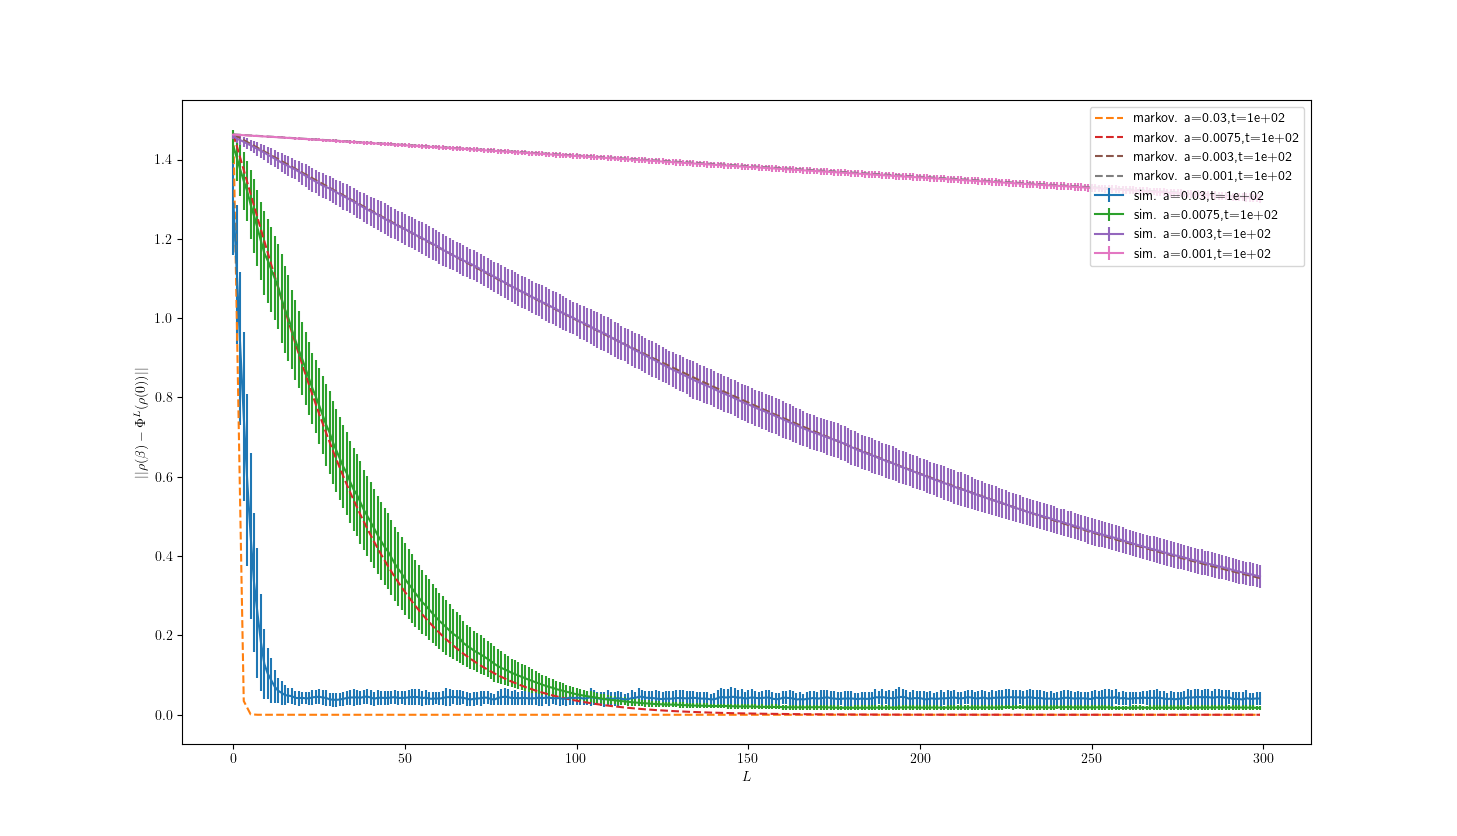
\includegraphics[width=0.45\linewidth]{numerics/data/sho_error_vs_l.png}
    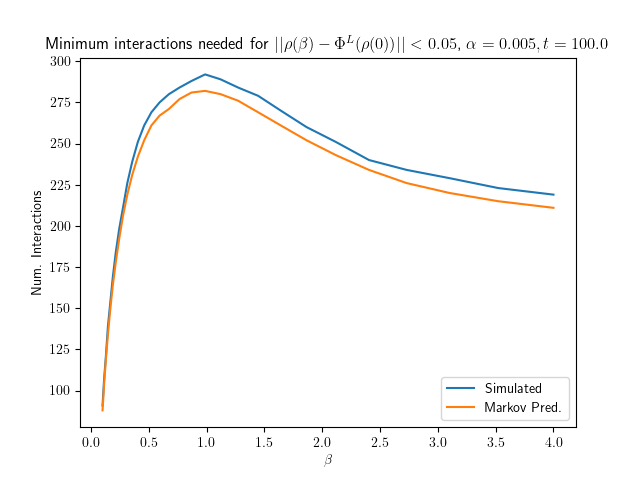
\includegraphics[width=0.45\linewidth]{numerics/data/sho_l_vs_beta.png} \\
    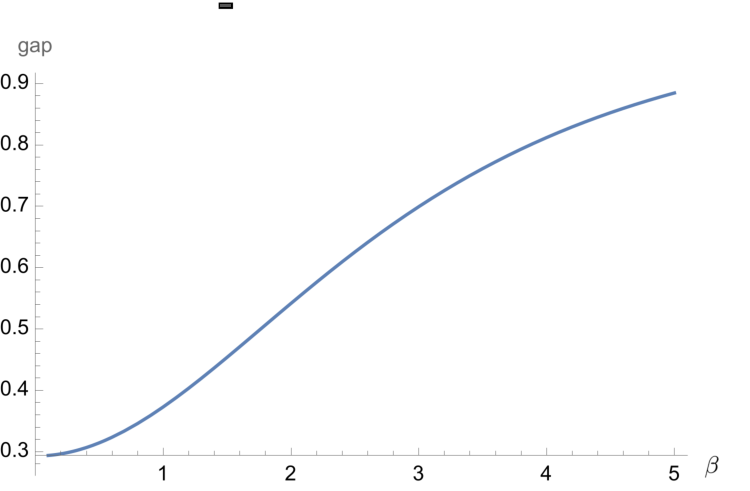
\includegraphics[width=0.5\linewidth]{numerics/data/spec_gap_dim_4.pdf}
    \caption{TODO: Improve. Trace distance to target as a function of interaction number, simulation compared to Markov chain behavior. The Hilbert-Schmidt overlap with the ground state $\anglebrackets{\Phi^L(\rho(0)), \ketbra{0}{0}}$ is 0.940 at $L = 300$. }
    \label{fig:enter-label}
\end{figure}

The behavior of the fixed $\epsilon$ plot reveals a very interesting phenomenon where the number of interactions, and therefore total thermalization time, needed to reach the thermal state goes \emph{down} after a peak at about $\beta = 1.0$. This means colder temperatures can be reached quicker than some intermediate temperatures, assuming a starting state of the maximally mixed state. Our rationale for this behavior is that the spectral gap of the resulting Markov chain must increase with $\beta$ faster than the distance from $\rho(0)$ to $\rho(\beta)$ grows with $\beta$. This bears out when we plot the spectral gap as a function of $\beta$ for the truncated harmonic oscillator, seen in Fig. \ref{fig:enter-label}.

Once we have determined how the thermalization process behaves for a given $\alpha$ and $t$, we can then sweep these parameters to determine how they effect thermalization. From our analysis of the single qubit case we would expect that the distance to the Markov chain can be made arbitrarily close as we both reduce the off-resonant terms by making $\alpha$ smaller and reducing the norm of the remainder terms by making $\widetilde{\alpha}$ smaller. As $t$ is not set we can choose which one to reduce by also varying $t$. As $t$ dictates the simulation time for the system dynamics we would like to reduce it as much as possible. The plot povided in Fig \ref{fig:total_time_vs_time} shows that the total simulation time tends to decrease as $t$ increases until some threshold is met. Finding this optimum value analytically would be intractable for arbitrary dimension harmonic oscillators. One other main takeaway is that as $\alpha$ increases the total simulation time also tends to decrease for a significant range of $t$. This is due to the fact that the probability mass that can be moved by the Markov chain increases with $\alpha$. We did not take this to the extreme and study a strong-coupling, short-time interaction channel and leave these questions for future research. 

\begin{figure}
    \centering
    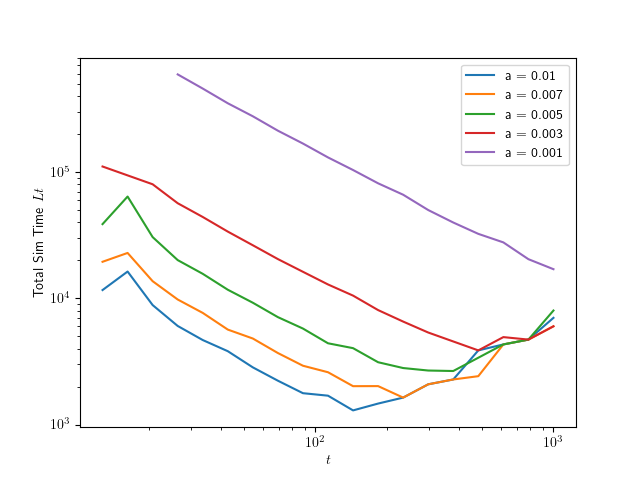
\includegraphics[width=0.75\linewidth]{numerics/data/total_time_vs_time.png}
    \caption{Total simulation time as a function of per-interaction simulation time $t$.}
    \label{fig:total_time_vs_time}
\end{figure}

\matt{Should we include some kind of dimension dependent behavior for oscillator numerics? What would be a good candidate to plot?}

\section{General Systems}
 Now that we have studied a single qubit and the harmonic oscillator in as much detail as possible, in this section we explore the behavior of our algorithm for some more generic systems. As our algorithm ultimately boils down to a Markov chain over the eigenstates of the Hamiltonian we are unable to make any runtime claims, as that would require bounding the spectral gap of a Markov chain that depends on knowledge of the Hamiltonian eigenvalues. What we do show in this section is three-fold: we first demonstrate that if the environment temperature approaches 0 ($\beta \to \infty$), then the ground state of the system is \emph{a} fixed point, second that if the eigenvalue differences $\lambda(i) - \lambda(j)$ can be sampled from exactly then we show that by taking $t$ sufficiently large the thermal state is the unique fixed point, and lastly we demonstrate that knowledge of eigenvalue gaps is largely an artifact of theory by preparing low temperature thermal states for Hydrogen chains without any a-priori knowledge.
 
% For a generic system it becomes very difficult to make any results without promises about our knowledge of the Hamiltonian. Right away the most obvious problem is that without prior knowledge we have no clue really what value of $\gamma$ we should tune our ancilla qubits to. For the single qubit and harmonic oscillator case we had complete knowledge of the spectrum of $H_S$. One thing we would like to show is that it is possible to do so if we also know the spectrum of $H_S$ completely. This will involve randomly choosing a value of $\gamma$ from the Bohr frequency set with importance sampling. Even with these promises it turns out to be incredibly difficult to analyze the resulting Markov chain for an arbitrary $\beta$. What we will do instead of an arbitrary thermal state preparation is to instead prepare the ground state. As an additional preprocessing step one could apply a filter function like a Heaviside step function to the Hamiltonian, thus eliminating the need for knowledge of eigenvalue gaps. This route was analyzed using Quantum Signal Processing (QSP) techniques in (Cite Danial dynamical cooling). 

We first briefly discuss what happens in the $\beta \to \infty$ limit. In this scenario our ancilla qubit is in the ground state, meaning that any transition that occurs must increase the energy of the ancilla and decrease the energy of the system. Since the ground state is the lowest possible energy, intuitively we would expect that no transitions out of the ground state occur and the ground state should remain fixed. This intuition is captured in the theorem below, where we ignore the effects of controllable off-resonant transitions and order $(\alpha t)^3$ contributions.
\begin{theorem}[Ground State Fixed Point] \label{thm:ground_state_fixed}
    For an arbitrary Hamiltonian $H$ and environment energy gap $\gamma$, in the limit as $\beta \to \infty$ the ground state of $H$ is a fixed point of the on-resonance second order dynamics. Formally,
    \begin{equation}
        \lim_{\beta \to \infty} (\identity + \mathcal{T}_{\on})(\ketbra{0}{0}) = \ketbra{0}{0}.
    \end{equation}
\end{theorem}
\begin{proof}
    To prove this we only have to show that $\lim_{\beta \to \infty} \mathcal{T}_{\on}(\ketbra{0}{0}) = 0$. Suppose $\gamma$ is sufficiently close to the eigenvalue difference $\lambda(j) - \lambda(0)$. Using Eq. \eqref{eq:on_resonance_transitions} from Lemma \ref{thm:second_order_transition} the on-resonance transition amplitude is
    \begin{align}
        \lim_{\beta \to \infty} \bra{j} \mathcal{T}_{\on}(\ketbra{0}{0}) \ket{j} &= \lim_{\beta \to \infty} \widetilde{\alpha}^2 \frac{e^{-\beta \gamma}}{1 + e^{-\beta \gamma}} \sinc^2 \left( \frac{(\Delta(j,0) - \gamma)t}{2} \right) = 0.
    \end{align}
    Since this holds for any $\gamma$ that produces an on-resonance transition we are done.
\end{proof}

Now we move on to showcase a scenario when finite $\beta$ thermal states are the unique fixed point of the Markov dynamics. For this we assume sample access to the eigenvalue differences $\Delta(i,j) = \lambda(i) - \lambda(j)$, meaning if there are $\chi(i,j)$ pairs of eigenvalues with positive differences $\Delta(k,l) = \Delta(i,j) \ge 0$ then the probability we receive $\Delta(i,j)$ is $\prob{\gamma = \Delta(i,j)} = \chi(i,j) \frac{2}{\dim_S(\dim_S - 1)}$. One simplifying assumption we will make (I'm not sure this is necessary?) is that there are no degeneracies in the Hamiltonian and for all $i,j$ we have $\Delta(i,j) > 0$. By taking $t$ larger than the smallest difference between eigenvalue differences we can ensure that the probability of an on-resonance transition occurring between states $i$ and $j$ is $\chi(i,j) \frac{2}{\dim_S(\dim_S - 1)}$. More formally, we use the definition of $\delta_{\min}$ from Eq. \eqref{eq:delta_min_def} and take $t \ge 1/ \delta_{\min}$ so that we can use Lemma \ref{lem:sinc_poly_approx} to argue that the only contribution to $\bra{j} \mathcal{T}_{\on}(\ketbra{i}{i}) \ket{j}$ is from $\gamma = \Delta(i,j)$. As $\gamma$ is a random variable this makes the transition coefficient a random variable as well. 

\begin{theorem}[Generic System Thermal State Fixed Point]
    Let $H_S$ be an Hermitian matrix with no degenerate eigenvalues, let $\chi(i,j)$ denote the number of eigenvalue differences of value $\Delta(i,j)$, and let $\gamma$ be a random variable with distribution $\prob{\gamma = \Delta(i,j)} = \frac{\chi(i,j)}{\binom{\dim_S}{2}}$. The thermal state $\rho_S(\beta) = \frac{e^{-\beta H_S}}{\partfun(\beta)}$ is the unique fixed point of the Markov chain dynamics of the thermalizing channel $\Phi$ in expectation with respect to $\gamma$, formally
    \begin{align}
        \mathbb{E}_{\gamma} \left[ (\identity + \mathcal{T}_{\on})(\rho_S(\beta)) \right] = \rho_S(\beta).
    \end{align}
    Combined with Jerison's Markov Relaxation Theorem \ref{thm:markov_chain_bound} this implies there exists sufficiently large $L_\star$ and $t$, along with a sufficiently small $\alpha$, such that for all starting states $\rho$ that are diagonal in the $H_S$ basis and for all $\epsilon > 0$
    \begin{equation}
    \norm{\rho_S(\beta) - (\mathbb{E}_\gamma \Phi_\gamma)^{\circ L_\star}(\rho)}_1 \le \epsilon.
    \end{equation}
\end{theorem}

\begin{proof}
For $j > i$ we have $\bra{j} \mathcal{T}_{\on}(\ketbra{i}{i}) \ket{j} = \widetilde{\alpha}^2 q(1; i, j) \mathbf{I}[\gamma = \Delta(i,j)]$ and for $j < i$ we have $\bra{j} \mathcal{T}_{\on}(\ketbra{i}{i}) \ket{j} = \widetilde{\alpha}^2 q(0; i, j) \mathbf{I}[\gamma = \Delta(i,j)]$. 

Now we can compute the expected on-resonance transition over this distribution of $\gamma$ for $i < j$ as
\begin{align}
    \mathbb{E}_{\gamma} \bra{j} \mathcal{T}_{\on}(\ketbra{i}{i}) \ket{j} &= \widetilde{\alpha} \mathbb{E}_{\gamma} q(1; i, j) \mathbf{I}[\gamma = \Delta(i,j)] \\
    &= \widetilde{\alpha}^2 \sum_{k > l} \prob{\gamma = \Delta(k,l)} q(1; i,j) \mathbf{I}[\Gamma = \Delta(i,j)] \\
    &= \widetilde{\alpha}^2 q(1; i,j) \frac{2 \chi(i,j)}{\dim_S(\dim_S - 1)}.
\end{align}
For $ i > j$ the same calculation follows but we replace $q(1; i, j)$ with $q(0;i,j)$ and for $i = j$ we just take the negative sum of all $i \neq j$ . This allows us to calculate the action of $\mathcal{T}_{\on}$ on the thermal state. In order for the thermal state to be a fixed point it must be in the kernel of $\mathcal{T}_{\on}$. To show this we will compute the overlap of the output with the ground state
\begin{align}
    &\mathbb{E}_{\gamma} \bra{0} \mathcal{T}_{\on}(\rho_S(\beta)) \ket{0} \nonumber \\
    &= \frac{1}{\partfun(\beta)} e^{-\beta \lambda(0)} \mathbb{E}_{\gamma} \bra{0} \mathcal{T}_{\on}(\ketbra{0}{0})\ket{0} + \frac{1}{\partfun(\beta)} \sum_{j > 0} e^{-\beta \lambda(j)} \mathbb{E}_{\gamma}  \bra{0} \mathcal{T}_{\on}(\ketbra{j}{j}) \ket{0} \\
    &= \frac{-1}{\partfun(\beta)} e^{-\beta \lambda(0)} \sum_{k > 0} \mathbb{E}_{\gamma} \bra{k} \mathcal{T}_{\on}(\ketbra{0}{0}) \ket{k} + \frac{1}{\partfun(\beta)} \sum_{j > 0} e^{-\beta \lambda(j)} \widetilde{\alpha}^2 q(0; 0, j) \frac{2 \chi(i,j)}{\dim_S (\dim_S - 1)} \\
    &= \frac{-1}{\partfun(\beta)} e^{-\beta \lambda(0)} \sum_{k > 0} \widetilde{\alpha}^2 q(1; 0, k) \frac{2 \chi(0, k)}{\dim_S(\dim_S - 1)} + \frac{1}{\partfun(\beta)} \sum_{j > 0} \widetilde{\alpha}^2 \frac{e^{-\beta \lambda(j)} }{1 + e^{-\beta \Delta(j, 0)}} \frac{2 \chi(0,j)}{\dim_S (\dim_S - 1)} \\
    &= \frac{2 \widetilde{\alpha}^2}{\partfun(\beta) \dim_S(\dim_S - 1)} \left(-\sum_{k > 0} e^{-\beta \lambda(0)} \frac{e^{-\beta \Delta(k, 0)}}{1 + e^{-\beta \Delta(k,0)}} \chi(0, k) + \sum_{j > 0} \frac{e^{-\beta \lambda(j)}}{1 + e^{-\beta \Delta(j, 0)}} \chi(0, j) \right) \\
    &= 0,
\end{align}
where we note that $e^{-\beta \lambda(0)} e^{-\beta \Delta(k, 0)} = e^{-\beta \lambda(k)}$ and we simply relabel the left summation index $k \mapsto j$, which then cancels with the other sum giving 0.

We now repeat the above calculation for the transition amplitude to the states in the middle with $0 < j < \dim_S - 1$. The main difference with this calculation is that we now have to split our summation into states with higher or lower energy than the input states. 
\begin{align}
    &\mathbb{E}_{\gamma} \bra{j} \mathcal{T}_{\on}(\rho_S(\beta)) \ket{j} \nonumber \\
    &= \frac{1}{\partfun(\beta)} \sum_{k < j} e^{-\beta \lambda(k)} \mathbb{E}_{\gamma} \bra{j} \mathcal{T}_{\on}(\ketbra{k}{k}) \ket{j} + \frac{e^{-\beta \lambda(j)}}{\partfun(\beta)} \mathbb{E}_{\gamma}\bra{j} \mathcal{T}_{\on} (\ketbra{j}{j}) \ket{j} + \frac{1}{\partfun(\beta)} \sum_{k > j} e^{-\beta \lambda(k)} \mathbb{E}_{\gamma} \bra{j} \mathcal{T}_{\on} (\ketbra{k}{k}) \ket{j}. \label{eq:generic_system_fixed_point_1}
\end{align}
We then can break down the middle self-transition term as the negative sum over the other transition elements as
\begin{align}
    \frac{e^{-\beta \lambda(j)}}{\partfun(\beta)} \mathbb{E}_{\gamma}\bra{j} \mathcal{T}_{\on} (\ketbra{j}{j}) \ket{j} &= - \frac{e^{-\beta \lambda(j)}}{\partfun(\beta)} \sum_{l < j} \mathbb{E}_{\gamma} \bra{l} \mathcal{T}_{\on} (\ketbra{j}{j}) \ket{l} - \frac{e^{-\beta \lambda(j)}}{\partfun(\beta)} \sum_{l > j} \mathbb{E}_{\gamma} \bra{l} \mathcal{T}_{\on} (\ketbra{j}{j}) \ket{l} \\
    &= -  \frac{2 \widetilde{\alpha}^2 e^{-\beta \lambda(j)} }{\partfun(\beta) \dim_S(\dim_S - 1)} \left( \sum_{l < j} q(0; l, j) \chi(l, j) + \sum_{l > j} q(1; l, j) \chi(l, j) \right) \\
    &= -  \frac{2 \widetilde{\alpha}^2  }{\partfun(\beta) \dim_S(\dim_S - 1)} \left( \sum_{l < j} \frac{e^{-\beta \lambda(j)}}{1 + e^{-\beta \Delta(j, l)}} \chi(l, j) + \sum_{l > j} \frac{e^{-\beta \lambda(l)}}{1 + e^{-\beta \Delta(l, j)}} \chi(l, j) \right). \label{eq:generic_system_fixed_point_2}
\end{align}
Now we can return to Eq. \eqref{eq:generic_system_fixed_point_1} and compute the expectation values within the sums as
\begin{align}
    \frac{1}{\partfun(\beta)} \sum_{k < j} e^{-\beta \lambda(k)} \mathbb{E}_{\gamma} \bra{j} \mathcal{T}_{\on}(\ketbra{k}{k}) \ket{j} &= \frac{2 \widetilde{\alpha}^2 }{\partfun(\beta) \dim_S(\dim_S - 1) } \sum_{k < j} e^{-\beta \lambda(k)} \frac{e^{-\beta \Delta(j, k)}}{1 + e^{-\beta \Delta(j, k)}} \chi(j, k) \\
    &= \frac{2 \widetilde{\alpha}^2 }{\partfun(\beta) \dim_S(\dim_S - 1) } \sum_{k < j} \frac{e^{-\beta \lambda(j)}}{1 + e^{-\beta \Delta(j, k)}} \chi(j, k), \label{eq:generic_system_fixed_point_3}
\end{align}
and likewise
\begin{align}
    \frac{1}{\partfun(\beta)} \sum_{k > j} e^{-\beta \lambda(k)} \mathbb{E}_{\gamma} \bra{j} \mathcal{T}_{\on}(\ketbra{k}{k}) \ket{j} &= \frac{2 \widetilde{\alpha}^2 }{\partfun(\beta) \dim_S(\dim_S - 1) } \sum_{k < j} e^{-\beta \lambda(k)} \frac{1}{1 + e^{-\beta \Delta(k, j)}} \chi(j, k). \label{eq:generic_system_fixed_point_4}
\end{align}
After relabeling summation indices, it is clear that adding Eqs. \eqref{eq:generic_system_fixed_point_2}, \eqref{eq:generic_system_fixed_point_3}, and \eqref{eq:generic_system_fixed_point_4} is equal to \eqref{eq:generic_system_fixed_point_1} and that therefore $0 < j < \dim_S - 1 \implies \bra{j} \mathcal{T}_{\on}(\rho_S(\beta)) \ket{j} = 0$.

To prove that the final transition amplitude is 0 we can use the fact that the trace of the on-resonance map is 0
\begin{align}
    \trace{\mathcal{T}_{\on}(\rho_S(\beta))} &= \sum_j \bra{j} \mathcal{T}_{\on}(\rho_S(\beta)) \ket{j} = 0\\
    \implies \bra{\dim_S - 1} \mathcal{T}_{\on}(\rho_S(\beta)) \ket{\dim_S - 1} &= - \sum_{j < \dim_S - 1} \bra{j} \mathcal{T}_{\on}(\rho_S(\beta)) \ket{j} \\ 
    &= 0.
\end{align}
This completes the proof that $\rho_S(\beta)$ is a fixed point of $\identity + \mathbb{E}_{\gamma} \mathcal{T}_{\on}$. To see that it is the unique fixed point we need to show ergodicity of the Markov chain $I + T$. The condition of ergodicity requires that the expected hitting time of any target state $j$ from any initial state $i$ is finite. Given our assumption of sample access to the $\Delta(i,j)$ distribution we have 
\begin{align}
    \bra{j} (\identity + \mathbb{E}_{\gamma} \mathcal{T}_{\on})(\ketbra{i}{i}) \ket{j} &= |\braket{j}{i}|^2 + \mathbb{E}_{\gamma} \bra{j} \mathcal{T}_{\on} (\ketbra{i}{i}) \ket{j}.
\end{align}
If $i = j$ the result is on the order of $1 - \Theta(\widetilde{\alpha}^2 \frac{2}{\dim_S (\dim_S - 1)})$, which approaches 1 as $\widetilde{\alpha} \to 0$, and is clearly greater than zero. If $i < j$ the result is $\frac{2 \widetilde{\alpha}^2}{\dim_S (\dim_S - 1)} q(1; i,j) \chi(i,j)$ which is positive. If $i > j$ the result is $\frac{2 \widetilde{\alpha}^2}{\dim_S (\dim_S - 1)} q(0; i,j) \chi(i,j)$ which again is positive. These three results show that for all $i$ and $j$ there is a nonzero probability of transitioning from $i$ to $j$ within a single interaction, meaning the expected hitting time is finite. This is sufficient for ergodicity and therefore uniqueness of the fixed point.

Lastly, we need to argue that there exist parameters that are sufficient for thermalization. As $\norm{\mathcal{T}_{\off}}_1 \le \frac{4 \alpha^2}{\delta_{\min}^2}$ and $\norm{R_{\Phi}}_1 \in \bigo{\alpha^3 t^3}$ there exists a small enough value of $\alpha$ such that $L_{\star}(\norm{\mathcal{T}_{\off}}_1 + \norm{R_{\Phi}}_1) \le \epsilon / 2$. The Markov Relaxation Theorem \ref{thm:markov_chain_bound} tells us that taking $L_{\star}$ sufficiently large yields $\norm{\rho_S(\beta) + (\identity + \mathbb{E}_{\gamma} \mathcal{T}_{\on})^{\circ L_{\star}}(\rho)}_1 \le \epsilon /2$. This completes the proof.
\end{proof}

One of the main drawbacks to our results thus far has been that the runtime depends on the spectral gap of a Markov chain, which in turn varies based on our knowledge of the eigenvalue differences $\Delta_S(i,j)$. Although characterizing this dependency analytically seems incredibly difficult, it is rather straightforward to test how well it works numerically on small, classically simulable systems. We did just this for two Hydrogen chain systems, H2 and H3, which are a standard benchmark system in computational chemistry. For each interaction we sample a value of $\gamma$ from a Gaussian distribution with mean $\trace{H_S}$ and variance $\frac{|\norm{H_S} - \trace{H_S}}{2}$, the trace is relatively easy to compute and $\norm{H_S}$ can typically be upper bounded. We then tracked the distance of the system state with each interaction and see a decrease in the error as the number of interactions proceeds. We observe that this rather oblivious distribution of $\gamma$ leads to surprisingly good results for conservative values of $\alpha = 10^{-3}$ and $t = 10^2$; we achieve a trace distance of 0.06 to the thermal state for $\beta = 3$ for H2 and $0.1$ for H3. See Fig. \ref{fig:h_chain_error} for results.
\begin{figure}
    \centering
    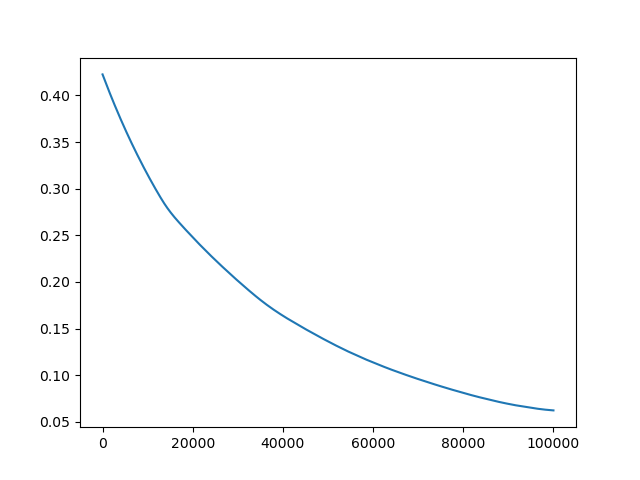
\includegraphics[width=0.45\linewidth]{numerics/data/h2_chain_2.png}
    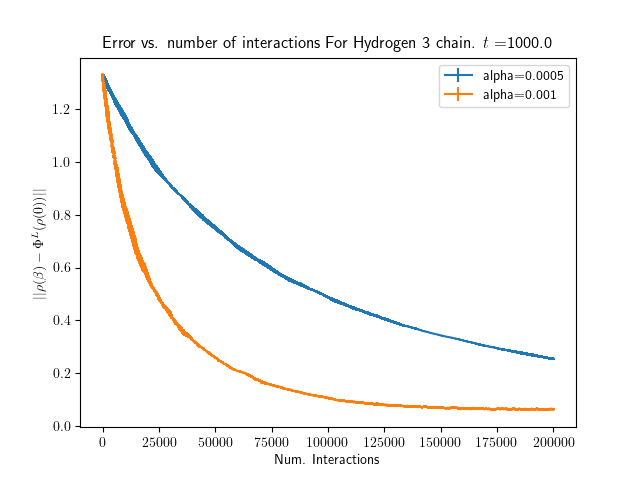
\includegraphics[width = 0.45\linewidth]{numerics/data/h3_chain_7.png}
    \caption{Hydrogen-2 and Hydrogen-3 chain distance to thermal state vs number of interactions. YES THIS IS A BAD PLOT IT NEEDS TO BE RERAN WITH LABELS.}
    \label{fig:h_chain_error}
\end{figure}

\section{Conclusion}

We presented an analysis of the simplest thermalizing channel and show that it is a good candidate to prepare thermal states.

\bibliographystyle{unsrt}
\bibliography{bib}

\appendix



\section{Sinc Function}

\begin{lemma}[Sinc Function Bounds] \label{lem:sinc_poly_approx}
    For $\sinc^2\left( \frac{x t}{2} \right)$ and $\delta_{\min}$ as defined in Eq. \eqref{eq:delta_min_def}, we will make significant use of the following bounds:
    \begin{align}
        |x| \ge \delta_{\min} \implies \sinc^2 \left( \frac{x t}{2} \right) &\le \frac{4}{\delta_{\min}^2 t^2} \label{eq:sinc_upper_bound} \\
        |x| \le \frac{\sqrt{2}}{t} \implies \sinc^2\left(\frac{x t}{2} \right) &\ge 1 - \frac{|x|^2 t^2}{2}. \label{eq:sinc_lower_bound}
\end{align}

\end{lemma}
\begin{proof}
    The first inequality is rather trivial
    \begin{align}
        \sinc^2 \left( \frac{x t}{2} \right) &= \frac{\sin^2 (x t /2)}{(x t / 2)^2} \le \frac{4}{x^2 t^2} \le \frac{4}{\delta_{\min}^2 t^2}.
    \end{align}
    The second involves a Taylor Series for $\sinc^2$, which we compute using the expression of $\sinc$ as $\sinc(x t/ 2) = \frac{\sin xt /2}{xt/2} = \int_0^1 \cos(sxt/2) ds$.  The first two derivatives can then be computed easily
    \begin{align}
        \frac{d \sinc^2(x t /2)}{dx} &= - t \int_0^1 \sin(sx) s ds \int_0^1 \cos(sx) ds \\
        \frac{d^2 \sinc^2(x t /2)}{dx^2} &= -t^2 / 2 \int_0^1 \cos(sx)s^2 ds \int_0^1 \cos(sx) ds + t^2 / 2 \int_0^1 \sin(sx) s ~ds \int_0^1 \sin(sx) s ~ds.
    \end{align}
    We can evaluate each of these derivatives about the origin using continuity of the derivatives along with the limits $\lim_{x \to 0} \cos(sx) = 1$ and $\lim_{x \to 0} \sin(sx) = 0$. We can now compute the mean-value version Taylor series as
    \begin{align}
        \sinc^2 \left(\frac{x t}{2} \right) &= \sinc^2(0) + x \frac{d}{dx} \sinc^2 \left(\frac{x t}{2} \right) \bigg|_{x = 0} + \frac{x^2}{2!} \frac{d^2}{dx^2} \sinc^2 \left(\frac{x t}{2} \right) \bigg|_{x = x_{\star}},
    \end{align}
    where $x_{\star} \in [0,1]$. 
    Plugging in $\sinc^2(0) = 1$ and $\frac{d\sinc^2(x t /2)}{dx}\big|_{x = 0} = 0$ then yields $|\sinc^2(xt/2) - 1| = \frac{|x|^2}{2} \abs{\frac{d^2\sinc^2(x t / 2)}{dx^2}\big|_{x = x_{\star}}}$. We make use of the rather simplistic bound
    \begin{align}
        \abs{\frac{d^2\sinc^2(sxt/2)}{dx^2}\bigg|_{x = x_{\star}} } &\leq t^2 / 2 \abs{\int_0^1 \cos(sx_{\star} t/ 2) s^2 ds \int_0^1 \cos(sx_{\star} t/ 2) ds} + t^2 /2 \abs{\int_0^1 \sin(sx_{\star} t/ 2) s ds \int_0^1 \sin(sx_{\star} t/ 2) s ds} \\
        &\leq t^2 / 2 \int_0^1 \abs{\cos(sx_{\star} t/2)} s^2 ds \int_0^1 \abs{\cos(sx_{\star} t /2 )} ds + t^2 / 2 \parens{\int_0^1 \abs{\sin(sx_{\star} t /2)} |s| ds}^2 \\
        &\leq t^2 / 2 \int_0^1 s^2 ds + t^2 / 2 \parens{\int_0^1 s ds}^2 \\
        &\leq t^2.
    \end{align}
    This yields the final inequality $|\sinc^2(x t /2 ) - 1| \leq \frac{|x|^2 t^2}{2}$ which yields Eq. \eqref{eq:sinc_lower_bound}.
\end{proof}


\section{Haar Integral Proofs} \label{sec:haar_integral_appendix}

In this section we present the more technical work needed to state our results in Section \ref{sec:taylor_series_phi}. The first two results are Lemmas that compute the effects of the randomized interaction in a form that are usable in the main result of Lemma \ref{lem:big_one}.

The first result we will make heavy use of can be found in a variety of places.
\begin{restatable}{lemma}{haar_two_moment} \label{lem:haar_two_moment}
    Let $\int (\cdot) dU$ denote the average distributed according to the Haar measure over $\dim$-dimensional unitary matrices $U$. Then for $\ket{i_1},\ket{i_2},\ldots,\ket{k_2}$ drawn from an orthonormal basis
    \begin{align}
        &\int \bra{i_1} U \ket{j_1} \bra{i_2} U \ket{j_2} \bra{k_1} U^\dagger \ket{l_1} ~ \bra{k_2} U^\dagger \ket{l_2} dU \nonumber \\
        &= ~\frac{1}{\dim^2 - 1} \parens{\delta_{i_1, l_1} \delta_{j_1, k_1} \delta_{i_2, l_2} \delta_{j_2, k_2} + \delta_{i_1, l_2} \delta_{j_1, k_2} \delta_{i_2, l_1} \delta_{j_2, k_1}} \nonumber \\
        &\quad - \frac{1}{\dim(\dim^2 - 1)} \parens{\delta_{i_1, l_2} \delta_{j_1, k_1} \delta_{i_2, l_1} \delta_{j_2, k_2} + \delta_{i_1, l_1} \delta_{j_1, k_2} \delta_{i_2, l_2} \delta_{j_2, k_1}}. \label{eq:haar_two_moment_integral}
    \end{align}
\end{restatable}

\begin{lemma} \label{lem:two_heisenberg_interactions}
    Let $G(t)$ denote the Heisenberg evolved random interaction $G(t) = e^{iHt} G e^{-iHt}$ for a total Hamiltonian $H$. After averaging over the interaction measure the product $G(x) G(y)$ can be computed as
    \begin{equation}
        \int G(x) G(y) dG = \frac{1}{\dim + 1} \parens{\sum_{(i,j),(k,l)} e^{i \Delta(i,j|k,l) (x-y)} \ketbra{i,j}{i,j} + \identity}.
    \end{equation}
\end{lemma}
\begin{proof}
The overall structure of this proof is to evaluate the product in the Hamiltonian eigenbasis and split the product into three factors: a phase contribution from the time evolution, a Haar integral from the eigenvalues of the random interaction, and the eigenvalue contribution of the random interaction. Since this involves the use of multiple indices, it will greatly simplify the proof to use a single index over the total Hilbert space $\hilb$ as opposed to two indices over $\hilb_S \otimes \hilb_E$. For example, the index $a$ should be thought of as a pair $(a_s, a_e)$, and functions $\lambda(a)$ should be thought of as $\lambda(a_s, a_e)$. Once the final form of the expression is reached we will substitute in pairs of indices for easier use of the lemma in other places.
    \begin{align}
        \int G(x) G(y) dG &= \int e^{+i H x} U_G D U_G^\dagger e^{-i H x} e^{+i H y} U_G D U_G^\dagger e^{-i H y} dU_G ~dD \\
        &= \int \bigg[\sum_a e^{+i \lambda(a)x}\ketbra{a}{a}  U_G \sum_b D(b)\ketbra{b}{b} U_G^\dagger \nonumber \\
        &\quad \sum_c e^{-i \lambda(c) (x - y)} \ketbra{c}{c} U_G \sum_d D(d)\ketbra{d}{d} U_G^\dagger \sum_e e^{-i \lambda(e) y} \ketbra{e}{e} \bigg] dU_G ~dD\\
        &=\sum_{a,b,c,d,e} \ketbra{a}{e} e^{-i (\lambda(c) - \lambda(a))x} e^{-i (\lambda(e) - \lambda(c))y} \nonumber \\
        &\quad \times \int \bra{a} U_G \ket{b} \bra{c} U_G \ket{d} \bra{b} U_G^{\dagger} \ket{c} \bra{d} U_G^\dagger \ket{e} dU_G \int D(b) D(d) dD \\
        &=  \sum_{a, b, c, d, e} \delta_{bd} \ketbra{a}{e} e^{-i (\lambda(c) - \lambda(a))x} e^{-i (\lambda(e) - \lambda(c))y} \nonumber \\
        &\quad \times \int \bra{a} U_G \ket{b} \bra{c} U_G \ket{d} \bra{b} U_G^{\dagger} \ket{c} \bra{d} U_G^\dagger \ket{e} dU_G. \\
    \end{align}
    Now the summation over $d$ fixes $d=b$ and we use Lemma \ref{lem:haar_two_moment} to compute the Haar integral, which simplifies greatly due to the repeated $b$ index. Plugging the result into the above yields the following
    \begin{align}
        &= \frac{1}{\dim^2 - 1} \sum_{a, b, c, e} \ketbra{a}{e} e^{-i (\lambda(c) - \lambda(a))x} e^{-i (\lambda(e) - \lambda(c))y} \parens{\delta_{ac} \delta_{ce} + \delta_{ae} - \frac{1}{\dim} \parens{\delta_{ac} \delta_{ce} + \delta_{ae}}}  \\
        &= \frac{1}{\dim^2 - 1} \parens{1 - \frac{1}{\dim}} \sum_{a, b, c, e} \ketbra{a}{e} e^{-i (\lambda(c) - \lambda(a))x} e^{-i (\lambda(e) - \lambda(c))y} \delta_{ae} (1 + \delta_{ac}) \\
        &= \frac{1}{\dim^2 - 1} \parens{1 - \frac{1}{\dim}} \sum_{a, b, c} \ketbra{a}{a} e^{i (\lambda(a) - \lambda(c))(x-y)} (1 + \delta_{ac}) \\
        &= \frac{1 \parens{\dim - 1}}{\dim^2 - 1} \sum_{a,c} \ketbra{a}{a} e^{i (\lambda(a) - \lambda(c))(x - y)} (1 + \delta_{ac}) \\
        &= \frac{1}{\dim + 1} \parens{\sum_{a,c} e^{i (\lambda(a) - \lambda(c))(x-y)} \ketbra{a}{a} + \identity}.
    \end{align}
    Reindexing by $a \mapsto i,j$, $c \mapsto k,l$, and plugging in the definition of $\Delta$ yields the statement of the lemma.
\end{proof}


\begin{lemma} \label{lem:sandwiched_interaction}
    Given two Heisenberg evolved random interactions, $G(x)$ and $G(y)$, we compute their action on an outer-product $\ketbra{i,j}{k,l}$ as
    \begin{equation}
        \int G(x) \ketbra{i,j}{k,l} G(y) ~dG = \frac{1}{\dim + 1} \parens{\ketbra{i,j}{k,l} + \braket{i,j}{k,l} \sum_{m,n} e^{i \Delta(m,n | i,j) (x-y)} \ketbra{m,n}{m,n}}
    \end{equation}
\end{lemma}
\begin{proof}
This proof is structured the same as Lemma \ref{lem:two_heisenberg_interactions} and similarly we will use a single index of the total Hilbert space $\hilb$ and switch to two indices to match the rest of the exposition.
    \begin{align}
        \int G(x) \ketbra{a}{b} G(y) dG &=  \int e^{i H x} U_G D U_G^{\dagger} e^{-i H x} \ketbra{a}{b} e^{i H y} U_G D U_G^\dagger e^{-i H y} ~dG \\
        &= \sum_{c, d, e, f} e^{i (\lambda(c) - \lambda(a))x} e^{i (\lambda(b) - \lambda(f))y} \nonumber \\
        &\quad \times \int \ketbra{c}{c} U_G D(d) \ketbra{d}{d} U_G^\dagger \ketbra{a}{b} U_G D(e) \ketbra{e}{e} U_G^\dagger \ketbra{f}{f} dG \\
        &= \sum_{c, d, e, f}  e^{i (\lambda(c) - \lambda(a))x} e^{i (\lambda(b) - \lambda(f))y} \ketbra{c}{f} \nonumber \\
        &\quad \times \int D(d) D(e) dD \int \bra{c} U_G \ket{d} \bra{b} U_G \ket{e} \bra{d} U_G^\dagger \ket{a} \bra{e} U_G^\dagger \ket{f} dU_G \\
        &=  \sum_{c,d,f} e^{i (\lambda(c) - \lambda(a))x} e^{i (\lambda(b) - \lambda(f))y} \ketbra{c}{f} \nonumber \\ 
        &\quad \times \int \bra{c} U_G \ket{d} \bra{b} U_G \ket{d} \bra{a} \overline{U_G} \ket{d} \bra{f} \overline{U_G} \ket{d} dU_G \\
        &= \frac{1}{\dim^2 - 1} \sum_{c,d,f} e^{i (\lambda(c) - \lambda(a))x} e^{i (\lambda(b) - \lambda(f))y} \ketbra{c}{f} (\delta_{ca} \delta_{bf} + \delta_{cf}\delta_{ab})\parens{1 - \frac{1}{\dim}} \\
        &= \frac{1}{\dim + 1} \sum_{c,f} e^{i (\lambda(c) - \lambda(a))x} e^{i (\lambda(b) - \lambda(f))y} \ketbra{c}{f} (\delta_{ca} \delta_{bf} + \delta_{cf}\delta_{ab}) \\
        &= \frac{1}{\dim + 1} \parens{\ketbra{a}{b} + \delta_{ab} \sum_{c} e^{i(\lambda(c) - \lambda(a))(x-y)} \ketbra{c}{c} }.
    \end{align}
    Now re-indexing by $a \mapsto (i,j)$, $b \mapsto (k,l)$ and $c \mapsto (m,n)$ results in the expression given in the statement of the lemma.
\end{proof}


\secondOrderChannelHaar*
\begin{proof}
To start we would like to note that we will use a single index notation to refer to the joint system-environment eigenbasis during this proof to help shorten the already lengthy expressions. We will convert back to a double index notation to match the statement of the theorem. We start from the expression for the first derivative of the channel $\frac{\partial}{\partial \alpha} \Phi_G(\rho_S)$ given by Eq. \eqref{eq:first_order_alpha_derivative}. To take the second derivative there are six factors involving $\alpha$, so we will end up with six terms. We repeat Eq. \eqref{eq:first_order_alpha_derivative} below, add a derivative, and label each factor containing an $\alpha$ for easier computation
\begin{align}
    \frac{\partial^2}{\partial \alpha^2} \Phi_G(\rho_S) =& \frac{\partial}{\partial \alpha} \parens{\int_{0}^{1} \underset{\substack{\downarrow \\ (A)}}{e^{i s (H+\alpha G)t}} (i t G) \underset{\substack{\downarrow \\ (B)}}{e^{i (1-s) (H+\alpha G)t}} ds ~ \rho \underset{\substack{\downarrow \\ (C)}}{e^{-i(H+\alpha G)t}} } \nonumber \\
    &~ ~+\frac{\partial}{\partial \alpha} \parens{ \underset{\substack{\downarrow \\ (D)} }{e^{i(H+\alpha G)t}} \rho \int_{0}^1 \underset{\substack{\downarrow \\ (E)} }{e^{-i s (H+\alpha G) t} } (- i t G) \underset{\substack{\downarrow \\ (F)}}{e^{-i (1-s) (H+\alpha G)t}} ds }. \label{eq:second_derivative_labels}
\end{align}
Our goal is to get each of these terms in a form in which we can use either Lemma \ref{lem:two_heisenberg_interactions} or \ref{lem:sandwiched_interaction}. 
\begin{align}
    (A) &=i t\int_0^1 \parens{\frac{\partial}{\partial \alpha} e^{i s_1 (H+ \alpha G)t}} G e^{i(1-s_1)(H+\alpha G)t} ds_1 \rho e^{-i (H+\alpha G)t} \bigg|_{\alpha=0} \\
    &= (it)^2 \int_0^1 \parens{\int_0^1 e^{i s_1 s_2 (H+\alpha G)t} s_1 G e^{i s_1 (1-s_2) (H+\alpha G)t} ds_2} G e^{i(1-s_1) (H+\alpha G)t} ds_1 \rho e^{-i(H+\alpha G) t} \bigg|_{\alpha=0} \label{eq:second_order_deriv_intermediate_a}\\
    &= -t^2 \int_0^1 \int_0^1 e^{i s_1 s_2 H t} G e^{-i s_1 s_2 H t} e^{i s_1 H t} G e^{-i s_1 H t} s_1 ds_1 ds_2 e^{i H t} \rho e^{-i H t} \\
    &= -t^2 \int_0^1 \int_0^1 G(s_1 s_2 t) G(s_1 t) s_1 ds_1 ds_2 \rho(t). \label{eq:second_deriv_alpha_first_term}
\end{align}

\begin{align}
    (B) &= it \int_0^1 e^{i s_1 (H + \alpha G)t} G \frac{\partial}{\partial \alpha}\parens{e^{i(1-s_1)(H + \alpha G)t}} ds_1 \rho e^{-i(H + \alpha G) t} \bigg|_{\alpha = 0} \\
    &= (it)^2 \int_0^1 e^{i s_1 (H + \alpha G)t} G \parens{\int_0^1 e^{i(1-s_1)s_2 (H + \alpha G)t} (1-s_1) G e^{i(1 - s_1)(1 - s_2)(H + \alpha G)t} ds_2} ds_1 ~ \rho e^{-i ( H + \alpha G)t} \bigg|_{\alpha = 0} \\
    &= -t^2 \int_0^1 \int_0^1 e^{i s_1 H t} G e^{i(1-s_1)s_2 H t} G e^{i(1-s_1)(1-s_2) H t} (1-s_1) ds_1 ds_2 ~ \rho e^{-i H t}\\ 
    &= -t^2 \int_0^1 \int_0^1 e^{i s_1 H t} G e^{-i s_1 H t} e^{i(s_1 + s_2 - s_1 s_2) H t} G e^{-i (s_1 + s_2 - s_1 s_2) H t} (1-s_1) ds_1 ds_2 ~ \rho(t) \\
    &= -t^2 \int_0^1 \int_0^1 G(s_1 t) G((s_1 + s_2 - s_1 s_2)t) (1-s_1) ds_1 ds_2 ~ \rho(t)
\end{align}

\begin{align}
    (C) &= it \int_0^1 e^{i s (H + \alpha G)t} G e^{i(1-s) (H + \alpha G) t} ds ~\rho ~ \frac{\partial}{\partial \alpha} \parens{ e^{-i (H + \alpha G) t} } \bigg|_{\alpha = 0} \\
    &= (i t) (-it) \int_0^1 e^{i s (H + \alpha G)t} G e^{i (1 - s) (H + \alpha G)t} ds ~ \rho ~ \parens{ \int_0^1 e^{-i s (H + \alpha G)t} G e^{-i (1- s) ( H + \alpha G)t } ds}\bigg|_{\alpha = 0} \\
    &= + t^2 \parens{\int_0^1 e^{i s H t} G e^{-i s H t} ds} e^{i H t} \rho e^{-i H t} \parens{\int_0^1 e^{i (1-s) H t} G e^{-i (1-s) H t} ds} \\
    &= + t^2 \int_0^1 G(st) ds ~ \rho(t) \int_0^1 G((1-s)t) ds
\end{align}

\begin{align}
    (D) &= (-it) \frac{\partial}{\partial \alpha} \parens{e^{i(H + \alpha G)t}} \rho \int_0^1 e^{-i s (H + \alpha G)t} G e^{-i (1-s)(H + \alpha G)t} ds \bigg|_{\alpha = 0} \\
    &= t^2 \parens{\int_0^1 e^{i s (H+ \alpha G)t} G e^{i (1-s) (H + \alpha G)t}ds} \rho \int_0^1 e^{-i s (H + \alpha G)t} G e^{-i (1-s)(H + \alpha G)t} ds \bigg|_{\alpha = 0} \\
    &=  t^2 \int_0^1 e^{i s H t} G e^{-i s H t} ds ~\rho(t) \int_0^1 e^{i (1-s) H t} G e^{-i (1-s) H t} ds \\
    &= t^2 \int_0^1 G(st) ds ~ \rho(t) ~ \int_0^1 G((1-s)t) ds
\end{align}

\begin{align}
    (E) &= (-it) e^{i (H+ \alpha G) t} ~ \rho ~\int_0^1 \frac{\partial}{\partial \alpha} \parens{e^{-i s_1 (H + \alpha G)t}} G e^{-i (1-s_1)(H + \alpha G)t} ds_1 \bigg|_{\alpha = 0} \\
    &= - t^2 e^{i(H + \alpha G)t} ~ \rho ~\int_0^1 \parens{\int_0^1 e^{-i s_1 s_2 (H + \alpha G) t} (s_1 G) e^{-i s_1 (1-s_2) (H + \alpha G)t} ds_2} G e^{-i(1-s_1)(H + \alpha G)t} ds_1 \bigg|_{\alpha = 0} \\
    &= -t^2 e^{i H t} \rho e^{-i H t} \int_0^1 \int_0^1 e^{i (1 - s_1 s_2) H t} G e^{-i (s_1 - s_1 s_2)H t} G e^{-i (1-s_1)H t} s_1 ds_1 ds_2 \\
    &= -t^2 \rho(t) \int_0^1 \int_0^1 G((1- s_1 s_2) t) G((1-s_1)t) s_1 ds_1 ds_2
\end{align}

\begin{align}
    (F) &= (-it) e^{i(H + \alpha G) t} \rho \int_0^1 e^{-i s_1 ( H + \alpha G) t} G \frac{\partial}{\partial \alpha} \parens{ e^{-i (1-s_1) ( H +\alpha G)t}} ds_1 \bigg|_{\alpha = 0} \\
    &= (-it)^2 e^{i (H + \alpha G)t} \rho \int_0^1 e^{-i s_1 (H + \alpha G)t} G \parens{\int_0^1 e^{-i(1-s_1) s_2 (H + \alpha G)t} (1-s_1) G e^{-i(1-s_1) (1-s_2) (H + \alpha G) t} ds_2} ds_1 \bigg|_{\alpha = 0} \\
    &= -t^2 e^{-i H t} \rho e^{-i H t} \int_0^1 \int_0^1 e^{i (1- s_1) H t} G e^{-i (1-s_1) H t} e^{i (1-s_1)(1-s_2) H t} G e^{-i(1-s_1)(1-s_2) H t} (1-s_1) ds_1 ds_2 \\
    &= -t^2 \rho(t) \int_0^1 \int_0^1 G((1-s_1)t) G((1-s_1)(1 - s_2) t) (1-s_1)ds_1 ds_2
\end{align}

Now our goal is to compute the effects of averaging over the interaction $G$ on the above terms, starting with $(A)$. As this involves a lot of index manipulations, similarly to the proofs of Lemmas \ref{lem:two_heisenberg_interactions} and \ref{lem:sandwiched_interaction} we will use a single index for the total system-environment Hilbert space and switch back to a double index to state the results. We will make heavy use of Lemma \ref{lem:two_heisenberg_interactions}.
\begin{align}
    \int (A) dG &= -t^2 \int_0^1 \int_0^1 \int G(s_1 s_2 t) G(s_1 t) dG s_1 ds_1 ds_2 \rho(t) \\
    &= \frac{-t^2 }{\dim + 1} \int_0^1 \int_0^1 \parens{\sum_{i,j} e^{i (\lambda(i) - \lambda(j)) (s_1 s_2 t - s_1 t)} \ketbra{i}{i} + \identity} s_1 ds_1 ds_2 \rho(t) \\
    &= \frac{- t^2 }{\dim + 1} \parens{\sum_{i} \sum_{j : \lambda(i) \neq \lambda(j)} \int_0^1 \int_0^1 e^{i(\lambda(i) - \lambda(j))t (s_1 s_2 - s_1)} s_1 ds_1 ds_2 \ketbra{i}{i} + \sum_{i} \sum_{j : \lambda(i) = \lambda(j)}\frac{1}{2} \ketbra{i}{i} + \frac{1}{2} \identity} \rho(t) \\
    &= \frac{- t^2 }{\dim + 1} \parens{\sum_i \sum_{j : \lambda(i) \neq \lambda(j)} \frac{1 - i (\lambda(i) - \lambda(j))t - e^{-i (\lambda(i) - \lambda(j))t}}{t^2 (\lambda(i) - \lambda(j))^2} \ketbra{i}{i} + \frac{1}{2} \sum_{i} (\eta(i) + 1) \ketbra{i}{i} } \rho(t) \\
    &= \frac{- 1}{\dim + 1}\parens{\sum_{i} \sum_{j: \Delta_{ij} \neq 0} \frac{1 - i \Delta_{ij}t - e^{-i \Delta_{ij} t}}{\Delta_{ij}^2} \ketbra{i}{i} + \frac{t^2}{2} \sum_{i} (\eta(i) + 1)\ketbra{i}{i} } \rho(t)
\end{align}

We can similarly compute the averaged $(B)$ term:
\begin{align}
    \int (B) dG &= -t^2 \int_0^1 \int_0^1 \int G(s_1 t) G((s_1 + s_2 - s_1 s_2) t) dG (1-s_1) ds_1 ds_2 ~ \rho(t) \\
    &= \frac{- t^2 }{\dim + 1} \int_0^1 \int_0^1 \parens{\sum_{i,j} e^{i (\lambda(i) - \lambda(j))(s_1 s_2 - s_2) t} \ketbra{i}{i} + \identity} (1 -s_1) ds_1 ds_2 \rho \\
    &= \frac{- t^2 }{\dim + 1} \parens{\sum_{i} \sum_{j : \lambda(i) \neq \lambda(j)} \int_0^1 \int_0^1 e^{i(\lambda(i) - \lambda(j))t (s_1 s_2 - s_2)} (1 - s_1) ds_1 ds_2 \ketbra{i}{i} + \sum_{i} \sum_{j : \lambda(i) = \lambda(j)}\frac{1}{2} \ketbra{i}{i} + \frac{1}{2} \identity} \rho(t) \\
    &= \frac{- t^2 }{\dim + 1} \parens{\sum_i \sum_{j : \lambda(i) \neq \lambda(j)} \frac{1 - i (\lambda(i) - \lambda(j))t - e^{-i (\lambda(i) - \lambda(j))t}}{t^2 (\lambda(i) - \lambda(j))^2} \ketbra{i}{i} + \frac{1}{2} \sum_{i} (\eta(i) + 1) \ketbra{i}{i} } \rho(t) \\
    &= \frac{-1}{\dim + 1}\parens{\sum_{i} \sum_{j: \Delta_{ij} \neq 0} \frac{1 - i \Delta_{ij}t - e^{-i \Delta_{ij} t}}{\Delta_{ij}^2} \ketbra{i}{i} + \frac{t^2}{2} \sum_{i} (\eta(i) + 1)\ketbra{i}{i} } \rho(t),
\end{align}
which we note is identical to $\int (A) dG$. As terms $(C)$ and $(D)$ involve a different method of computation we skip them for now and compute $(E)$ and $(F)$. 
\begin{align}
    \int (E) dG &= -t^2 \rho(t) \int_0^1 \int_0^1 \int G((1- s_1 s_2) t) G((1-s_1)t) dG s_1 ds_1 ds_2 \\
    &= \frac{- t^2}{\dim + 1} \rho(t) \int_0^1 \int_0^1 \parens{\sum_{i,j} e^{i(\lambda(i) - \lambda(j)) t (s_1 - s_1 s_2)} \ketbra{i}{i} + \identity } s_1 ds_1 ds_2 \\
    &= \frac{- t^2}{\dim + 1} \rho(t) \parens{\sum_i \sum_{j : \lambda(i) \neq \lambda(j)} \frac{1 + i (\lambda(i) - \lambda(j))t - e^{i(\lambda(i) - \lambda(j))t}}{t^2 (\lambda(i) - \lambda(j))^2}\ketbra{i}{i} + \frac{1}{2} \sum_{i} (\eta(i) + 1 )\ketbra{i}{i}} \\
    &= \frac{- 1}{\dim + 1} \rho(t) \parens{\sum_i \sum_{j: (\Delta_{ij} \neq 0)} \frac{1 + i \Delta_{ij}t - e^{i\Delta_{ij}t}}{\Delta_{ij}^2} \ketbra{i}{i} + \frac{t^2}{2}\sum_i (\eta(i) + 1) \ketbra{i}{i}}.
\end{align}
Computing $(F)$ yields
\begin{align}
    \int (F) dG &= -t^2 \rho(t) \int_0^1 \int_0^1 \int G((1-s_1)t) G((1-s_1)(1 - s_2) t) dG (1-s_1)ds_1 ds_2 \\
    &= \frac{- t^2 \sigma ^2}{\dim + 1} \rho(t) \int_0^1 \int_0^1 \parens{\sum_{i,j} e^{i(\lambda(i) - \lambda(j))t (s_2 - s_1 s_2)}\ketbra{i}{i} + \identity} (1-s_1) ds_1 ds_2 \\
    &= \frac{- t^2 }{\dim + 1} \rho(t) \parens{\sum_{i} \sum_{j : \lambda(i) \neq \lambda(j)} \frac{1 + i (\lambda(i) - \lambda(j))t - e^{i (\lambda(i) - \lambda(j))t}}{t^2 (\lambda(i) - \lambda(j))^2} \ketbra{i}{i} +\frac{1}{2} \sum_{i} (\eta(i) + 1) \ketbra{i}{i}} \\
    &= \frac{- 1}{\dim + 1} \rho(t) \parens{\sum_i \sum_{j: (\Delta_{ij} \neq 0)} \frac{1 + i \Delta_{ij}t - e^{i\Delta_{ij}t}}{\Delta_{ij}^2} \ketbra{i}{i} + \frac{t^2}{2}\sum_i (\eta(i) + 1) \ketbra{i}{i}}
\end{align}
 which is identical to $\int (E) dG$.

 The last two terms $(C) = (D)$ are computed as follows:
 \begin{align}
     \int (C) dG &= t^2 \int_0^1 \int_0^1 \int G(s_1 t) \rho(t) G((1-s_2)t) ~dG ~ ds_1 ds_2 \\
     &= t^2 \sum_{i,j} \rho_{ij} e^{i(\lambda(i) - \lambda(j))t} \int_0^1 \int_0^1 \int G(s_1 t) \ketbra{i}{j} G((1-s_2)t) ~ dG ~ ds_1 ds_2 \\
     &= \frac{ t^2}{\dim + 1} \sum_{i,j} \rho_{ij} e^{i(\lambda(i) - \lambda(j))t} \parens{ \ketbra{i}{j} + \delta_{ij} \sum_{a} \int_0^1 \int_0^1 e^{i(\lambda(a) - \lambda(i))(s_1 + s_2 - 1)t} ds_1 ds_2 \ketbra{a}{a}} \\
     &= \frac{ t^2}{\dim + 1} \sum_{i,j} \rho_{ij} e^{i \Delta_{ij} t} \parens{\ketbra{i}{j} + \delta_{ij} \sum_{a : \Delta_{ai} \neq 0} \frac{2( 1- \cos (\Delta_{ai} t))}{\Delta_{ai}^2 t^2} \ketbra{a}{a} + \delta_{ij} \sum_{a : \Delta_{ai} = 0} \ketbra{a}{a}}
 \end{align}

 We can now combine each of these terms to offer the full picture of the output of the channel to second order. We make two modifications to the results from each sum: first, we will switch to double index notation to make for easier use in other areas, and secondly we let $\rho = \ketbra{i,j}{k,l}$. We note that the first term in the following equation is provided by $(A) + (B)$, the second through $(E) + (F)$, and the last two through $(C) + (D)$. 
 \begin{align}
     &\int \frac{\partial^2}{\partial \alpha^2} \Phi_G(\ketbra{i,j}{k,l})\bigg|_{\alpha = 0} dG \\
     &= -\frac{2  e^{i \Delta(i,j|k,l) t}}{\dim + 1} \bigg(\sum_{(a,b): \Delta(i,j|a,b) \neq 0} \frac{1 - i \Delta(i,j|a,b)t - e^{-i \Delta(i,j|a,b) t}}{\Delta(i,j|a,b)^2} \nonumber \\
     &~+ \sum_{(a,b): \Delta(k,l|a,b) \neq 0} \frac{1 + i \Delta(k,l|a,b) t - e^{i \Delta(k,l|a,b) t}}{\Delta(k,l|a,b)^2} + \frac{t^2}{2}(\eta(i,j) + \eta(k,l)) \bigg) \ketbra{i,j}{k,l} \nonumber \\
    &~ +\delta_{i,k} \delta_{j,l} \frac{2 e^{i \Delta(i,j|k,l)t}}{\dim+1} \parens{ \sum_{(a,b): \Delta(i,j|a,b) \neq 0 } \frac{2(1- \cos (\Delta(i,j|a,b)t))}{\Delta(i,j|a,b)^2} \ketbra{a,b}{a,b} + t^2 \sum_{(a,b) : \Delta(i,j|a,b) = 0} \ketbra{a,b}{a,b}} \label{eq:second_order_output}
 \end{align}
The last step we need is to use the half angle formula to change the cosine to a sine
\begin{align}
    \frac{2(1 - \cos(\Delta(i,j| a,b)t)}{\Delta(i,j|a,b)^2} &= \frac{2\left( 1 - \left(1 - 2 \sin^2\left(\frac{\Delta(i,j|a,b)t}{2} \right) \right) \right)}{\Delta(i,j|a,b)^2} \label{eq:trig_start} \\
    &= t^2 \frac{\sin^2 \left(\frac{\Delta(i,j|a,b) t}{2} \right)}{\frac{\Delta(i,j|a,b)^2 t^2}{4}} \\
    &= t^2 \sinc^2 \left(\frac{\Delta(i,j|a,b) t}{2 } \right), \label{eq:trig_end}
\end{align}
which yields the statement.


We can compute these by plugging in to Eq. \eqref{eq:el_gigante} again, which yields
\begin{align}s
&\int \bra{i', j'} \mathcal{T} \left( \ketbra{i, j}{i, j} \right) \ket{i', j'} ~dG = \begin{cases}        
\widetilde{\alpha}^2 \sinc^2(\Delta(i,j | i', j') t /2) & (i, j) \neq (i', j') \\
            - \widetilde{\alpha}^2 \sum_{(a,b) \neq (i, j)} \sinc^2(\Delta(a,b|i,j) t / 2) & (i,j) = (i', j')
        \end{cases}. \label{eq:system_environment_transitions}
    \end{align}
    The $(i, j) \neq (i', j')$ case should be apparent, the first term with the coherence factors $\chi$ are zero and the second term is what remains. The $(i,j) = (i', j')$ case can be seen as follows. For the first term we have
    \begin{align}
        - \frac{\alpha^2 e^{i \Delta(i,j| i,j) t}}{\dim + 1}\left(\chi(i,j) + \chi(i,j)^* + \frac{t^2}{2}(\eta(i,j) + \eta(i,j) \right) \ketbra{i,j}{i,j}.
    \end{align}
    We first compute the sum $\chi(i,j) + \chi(i,j)^*$ as
    \begin{align}
        \chi(i,j) + \chi(i,j)^* &= \sum_{a,b: \Delta(i,j,|a,b) \neq 0} \frac{1 - i \Delta(i,j|a,b)t - e^{-i \Delta(i,j|a,b) t}}{\Delta(i,j|a,b)^2} \nonumber\\
&\quad+ \sum_{a,b: \Delta(i,j,|a,b) \neq 0} \frac{1 + i \Delta(i,j|a,b)t - e^{+i \Delta(i,j|a,b) t}}{\Delta(i,j|a,b)^2} \\
    &= \sum_{a,b: \Delta(i,j| a,b) \neq 0} \frac{2 - e^{-i \Delta(i,j| a,b) t} - e^{+i \Delta(i,j| a,b) t}}{\Delta(i,j|a,b)^2} \\
    &= \sum_{a,b: \Delta(i,j| a,b) \neq 0} t^2 \sinc^2 \left( \frac{\Delta(i,j| a,b) t}{2} \right),
    \end{align}
    where the last step follows from a trigonometric identity (see Eqs. \eqref{eq:trig_start} - \eqref{eq:trig_end} in Appendix \ref{sec:haar_integral_appendix} for details). Since $\sinc(0) = 1$ the $\eta(i,j)$ term can be expressed as $\eta(i,j) = \sum_{a,b : \Delta(i,j|a,b) = 0} \sinc^2 \left( \frac{\Delta(i,j| a,b) t}{2} \right)$. Plugging this into Eq. \eqref{eq:el_gigante} gives
    \begin{align}
        &\int \bra{i,j} \mathcal{T} (\ketbra{i,j}{i,j}) \ket{i,j} dG \\
        &= \bra{i,j} \left(-\frac{\alpha^2 t^2}{\dim + 1} \sum_{a,b} \sinc^2 \left( \frac{\Delta(i,j| a,b) t}{2} \right) \ketbra{i,j}{i,j} + \sum_{a,b} \sinc^2\left( \frac{\Delta(i,j | a,b)t}{2} \right) \ketbra{a,b}{a,b} \right) \ket{i,j} \\
        &= -\frac{\alpha^2 t^2}{\dim + 1} \sum_{(a,b) \neq (i,j)} \sinc^2 \left( \frac{\Delta(i,j| a,b) t}{2} \right).
    \end{align}
    As a by-product of this computation we have just shown that $\trace{\mathcal{T}(\rho)} = 0$ and that our mapping is trace preserving to $\bigo{\alpha^2}$.
\end{proof}





\end{document}